\chapter{Approach for identifying Microservices}
\label{ch:Solution}
This chapter presents an approach to tackle the issue of microservice identification. The process is partitioned in several steps, where each step is presented in its own section.
As noted in the \textit{State of the Art} (Chapter \ref{ch:StateOfTheArt}), existing approaches support two initial situations: They either conduct the extraction of microservices from existing (monolithic) systems or they are based on microservice greenfield development. Both types have their advantages and disadvantages. Existing systems, for instance, provide more information about the system specification and requirements. Legacy code and log files can be used to extract data dependencies or process structures. However, shortcomings in the design of the legacy application might have an impact on the extracted information and influence the microservice extraction in a negative manner. In contrast, greenfield development is not affected by any previously committed design decisions. As a matter of fact, the greenfield approach can be applied to existing systems as well, by discarding legacy code and additional information that arose during the development. Solely the system requirements that existed before the implementation started serve as input. Nevertheless, this type has to manage the identification process with less input.\\
The approach we propose is based on pre-existing system requirements. No existing implementation is used, consequently the presented approach is to be classified as greenfield method.\\



\section{Basic Approach}


\vspace{0.5cm}
\par
\begingroup
\leftskip=1cm
\rightskip=1cm

\noindent
\textbf{RQ1.1: Which is an appropriate strategy to decompose a system into microservices? }

\endgroup
\vspace{0.5cm}



\noindent
This thesis proposes a formal, graph-based microservice identification approach using clustering on control flow and data flow. It is  inspired by Amiri’s work on \textit{Object-aware Identification of Microservices} \cite{ObjectAwareAmiri}. In chapter \ref{ch:StateOfTheArt}, eight suitable approaches to identify microservices are presented and compared using well-defined criteria. Most of them require special prerequisites and cannot be applied to various types of systems, i.e. no greenfield applications, systems without meaningful VCS meta-data or the absence of log files.
\\
By the way of contrast, Amiri proposes an approach to extract structural and data object dependencies from business point of view in order to generate possible microservice candidates. In doing so, he relinquishes to use any further information besides BPMN models. Using both, structural and data object dependencies promotes high cohesiveness and loose coupling on functional and data object level. In other words, highly cohesive functionality is divided into the same microservices, together with the data objects that are accessed. \\
However, Sec.\ref{sec:stateOfTheArt:comparison} outlines the limitations and drawbacks of this approach. Whereas the control flow is depicted clearly, the data flow remains vague. The weight definitions regarding data object dependencies lack formal explanation. Further, the aggregation of structural and data object dependencies, and consequently the aggregation of control flow and data flow contains a significant problem: In Amiri's approach, the aggregation is conducted by summing up two relation matrices. The matrix entries representing the dependencies highly influence the results. For instance, a large amount of data reads and writes sum up to great numbers, outweighing the structural dependencies. Thus, the identification process would be almost based on data dependencies only, discarding any identified structural dependencies. \\
The following sections introduces a formal approach to tackle \textit{RQ1.2}. First, a basic overview of the approach is provided. Afterwards, each step is introduced in detail including alternatives and examples. 




\vspace{0.5cm}
\par
\begingroup
\leftskip=1cm
\rightskip=1cm

\noindent
\textbf{RQ1.2: What formal approach can be constructed to identify possible microservices without detailed know-how and manual effort? }

\endgroup
\vspace{0.5cm}



\noindent
To that end, Fig.\ref{fig:thesisProcess} provides an overview of the proposed approach. As depicted previously, the process requires input in form of BPMN models. Therefore, specifying those models marks the beginning of the process. Afterwards, control flow and data flow need to be extracted. To avoid the ambiguity of aggregating data flow and control flow as proposed by Amiri, the approach recommends to create two independent weighted Graphs, using the information from the previous step. In the next step, a clustering algorithm determines two sets of clusters based on the weights in the graphs. At that point, the process determined a set of clusters that is based on the control flow and another one, based on the data flow. In the following, a matching process identifies commonalities between data object-based and structural-based clusters in order to create comprehensive clusters. Based on these clusters, the last step extracts microservice candidates. \\

\textit{RQ2.1} also broaches the subject of necessary know-how and the amount of manual effort. As far as that is concerned, the proposed approach does not require human interaction as soon as the BPMN models are specified. Everything beyond that is based on a structural process.
Admittedly, the manual effort to conduct the process entirely is still not to be neglected, as the extraction process, graph creation and cluster matching is not yet automated. Nevertheless, the structural process enables to implement the entire approach, excluding the BPMN model specification step. However, implementing an approach is beyond the scope of the thesis.




 
\begin{figure}[h!]
	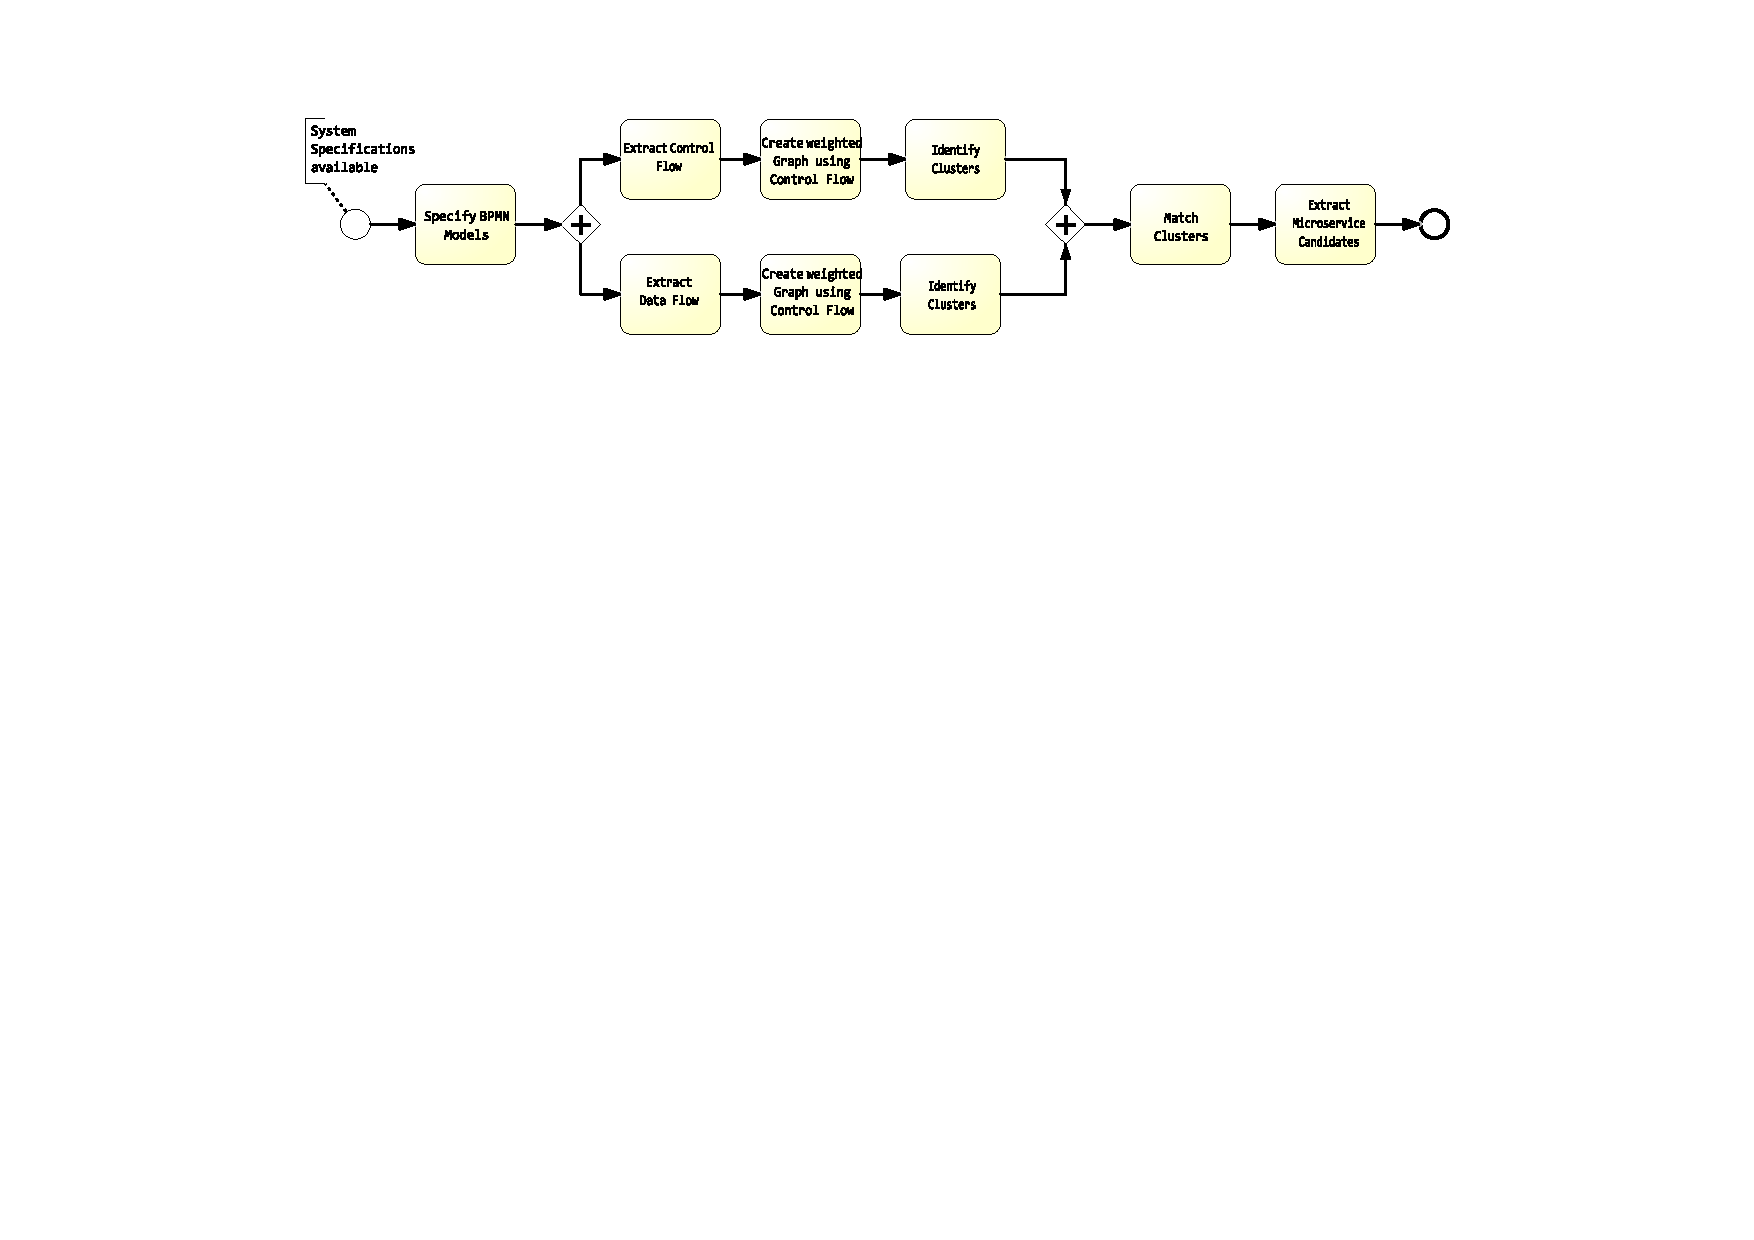
\includegraphics[width=\textwidth, trim={7.5cm 15.3cm 5.0cm 1.5cm}]{img/ThesisProcess.pdf}
	\caption{Overview of the identification approach}
	\label{fig:thesisProcess}
\end{figure}






\section{Specify BPMN Models}
\label{sec:Solution:SpecifyBPMN}
Chapter \ref{ch:background} introduces the BPMN 2.0 modelling language as an easy to use, but yet powerful notation to illustrate business processes including their activities and their data needs.
In the first step of the solution, those business processes need to be specified. Usually, the system specification are not directly given in form of business processes, but rather in the form of use cases, UML models, domain models or even as textual description in natural language. Therefore, the first step consists of specifying a business model using the available system specification. This can be achieved using various approaches, for instance: \\





\noindent
\textbf{Workshops} At the very beginning of a software project, technical and non-technical stakeholders can participate in a workshop to specify the business process model. As illustrated in the BPMN specification, the "primary goal of BPMN is to provide a notation that is readily understandable by all business users"  \cite{OMG}. Therefore, carrying out a workshop with stakeholders from various departments can produce high quality BPMN models which can be further used as input for the extraction process.\\
\textbf{Use Cases} In the case of CoCoME, the system specifications are available as use cases (cf. chapter \ref{ch:CoCoME}). 
Accordingly, section \ref{sec:PrepApproach:TransformUCtoBPMN} illustrates a process to transform use cases into BPMN models.  \\
\textbf{Others} Business processes can be extracted in various other ways. UML Activity diagrams, for instance, are very similar to BPMN models. Van der Aalst \textit{et al.} elaborated the Process Mining Manifesto \cite{ProcessMiningManifesto} where he presents general techniques to extract business processes, although it is mainly event log driven. Another approach is the \textit{BPMN Miner}, an automatic discovery tool for BPMN process models \cite{BPMNMiner}. Again, the tool discovers the models dynamically, using log files of a legacy system.





\subsection{Transform Use Case Sets in BPMN Processes}
\label{sec:PrepApproach:TransformUCtoBPMN}
To visualize the implicit data and control flow in use cases, it is necessary to transform the given use cases into BPMN models. In "Visualizing Use Case Sets as BPMN Processes" \cite{VisualizeBPMN}, Lübke \textit{et al.} already elaborated an approach to visualize the control flow that is hidden in use cases. As Lübke does not use the BPMN 2.0 notation, data is not considered and hence, data flow is not part of the given approach. In the following, we will introduce a conceptional approach, which is based on \cite{VisualizeBPMN}, to transform use cases into BPMN models:

\begin{figure}[h!]
	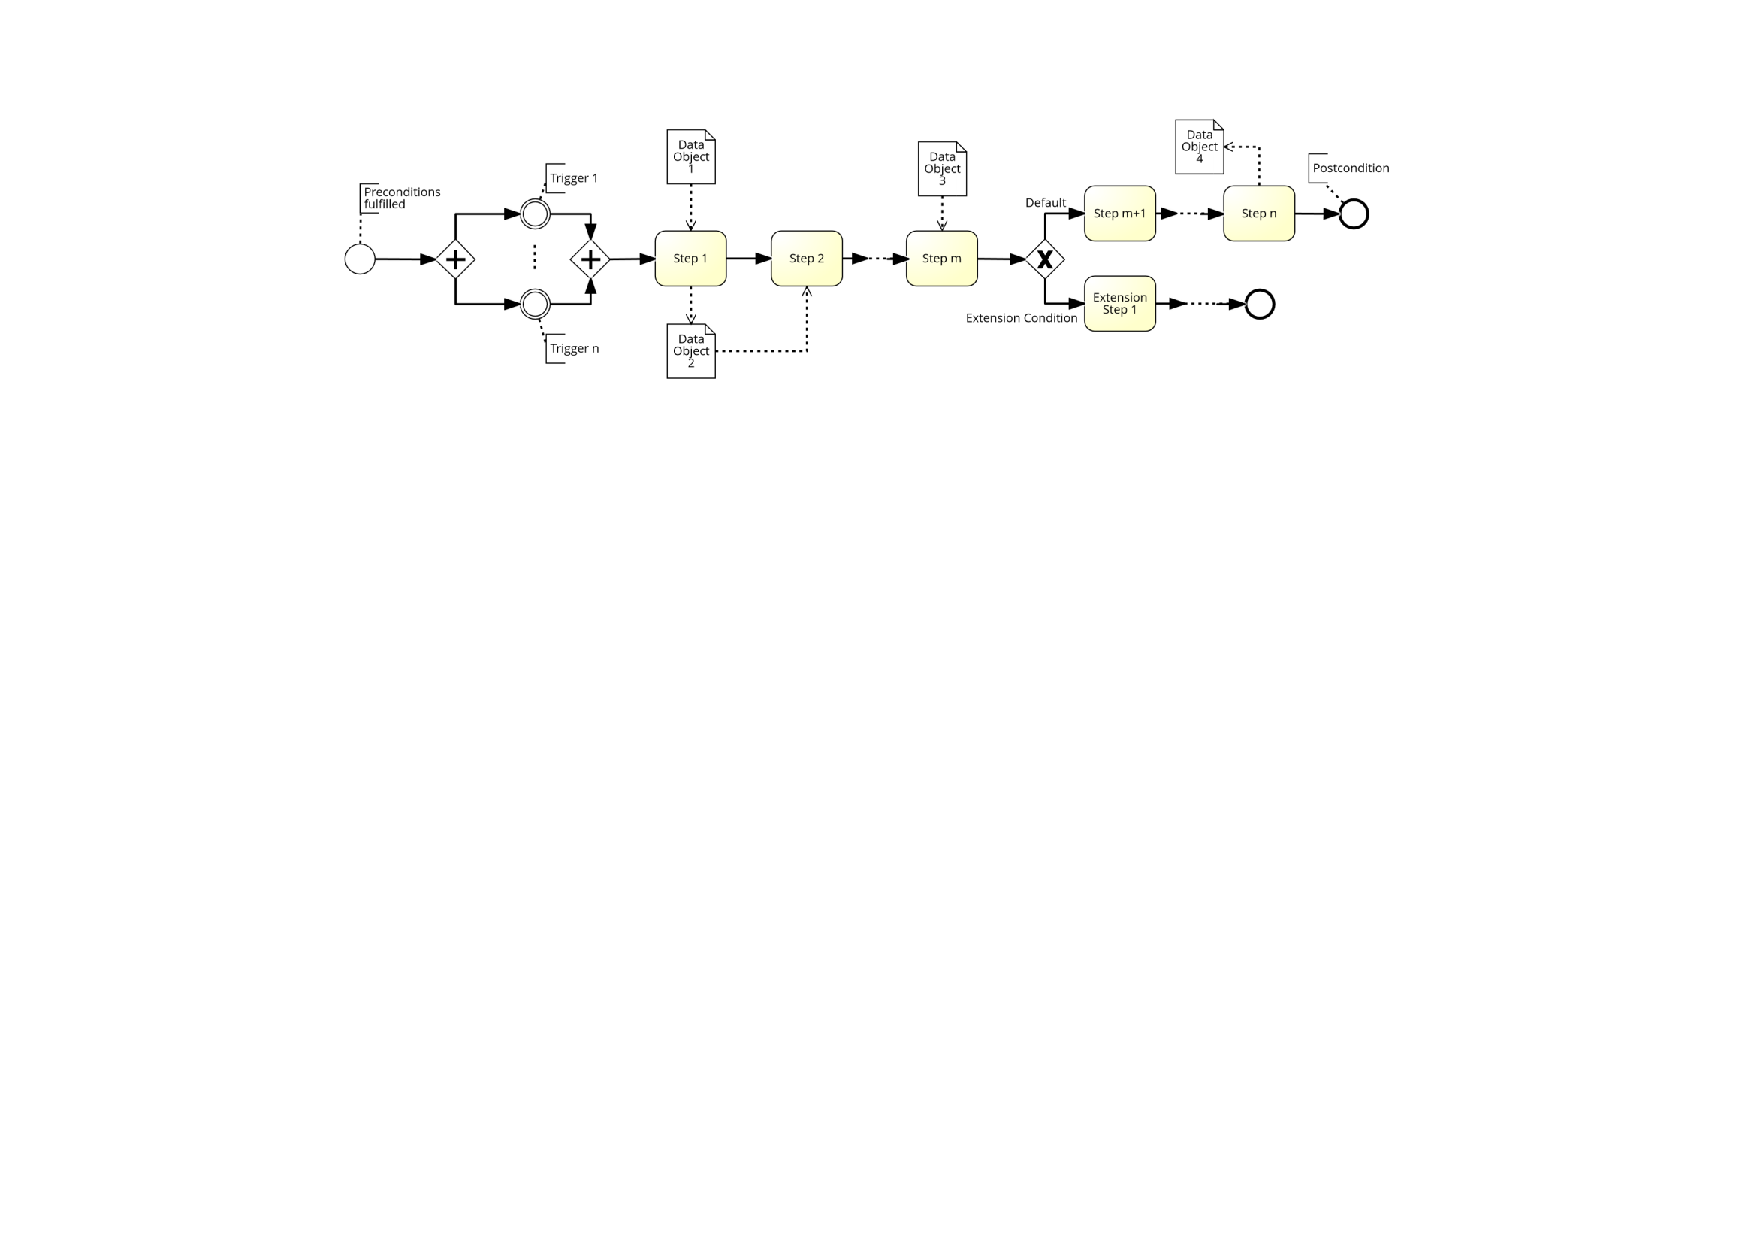
\includegraphics[width=\textwidth, trim={6cm 14.5cm 6cm 1.5cm}]{img/usecaseTransformation.pdf}
	\caption{Use Case transformed in a BPMN process}
	\label{fig:useCaseTransformation}
\end{figure}

\begin{enumerate}
	\item Create a flat use case model. Replace \textit{include} and \textit{extend} relationships by the associated use case
	\item Generate an independent BPMN process for each use case
	\item Join the generated BPMN processes based on preconditions, trigger and postconditions
	\item Remove duplicate Data Objects and refactor the data associations
	\item Refactor the business model i.e. divide or remove unnecessary steps, identify synonymous data objects, trigger etc.
\end{enumerate}


\noindent
The first step only includes simple substitutions, as the \textit{extend} and \textit{include} relationships simply have to be replaced by the actual use case.\\
Step number two represents the main part of the transformation. Fig.\ref{fig:useCaseTransformation} is an additional illustrative diagram that explains this step. First, the preconditions are assigned to the start event by using an annotation. Triggers are represented by intermediate events and as they are executed in parallel, connected by two Parallel Gateways. Each step in the use case's standard process is represented by a single task. This procedure might include some refactoring as further enlightened in the final step. Tasks that produce and/or consume data are connected to the corresponding data object. It has to be noticed, that data objects appear only once in a model. Given these point, it is necessary to check if a data object is already referenced by a previous task. Jumps and alternatives are modelled using Exclusive Or (XOR) Gateways. Finally, the postcondition is added as annotation and connected to the end event. \\
Joining the use case-based BPMN models is necessary to represent the control flow and data flow within the entire system. (The flows are generally not limited to "use case borders"). For each pair of use cases (\textit{UC A} and \textit{UC B}), check if the postcondition of UC A exists as precondition or trigger of UC B. If this is the case, join the accompanying BPMN processes by deleting the start event (BPMN process of UC B) and the end event (BPMN process of UC A) and connect the graphs. \\
In case that multiple use cases have the same postcondition, their BPMN processes are connected using an Exclusive Or Gateway (Fig.\ref{fig:JoinBPMNPostcondition}). 

\begin{figure}[h!]
	\centering
	\begin{minipage}{0.45\textwidth}
		\centering
		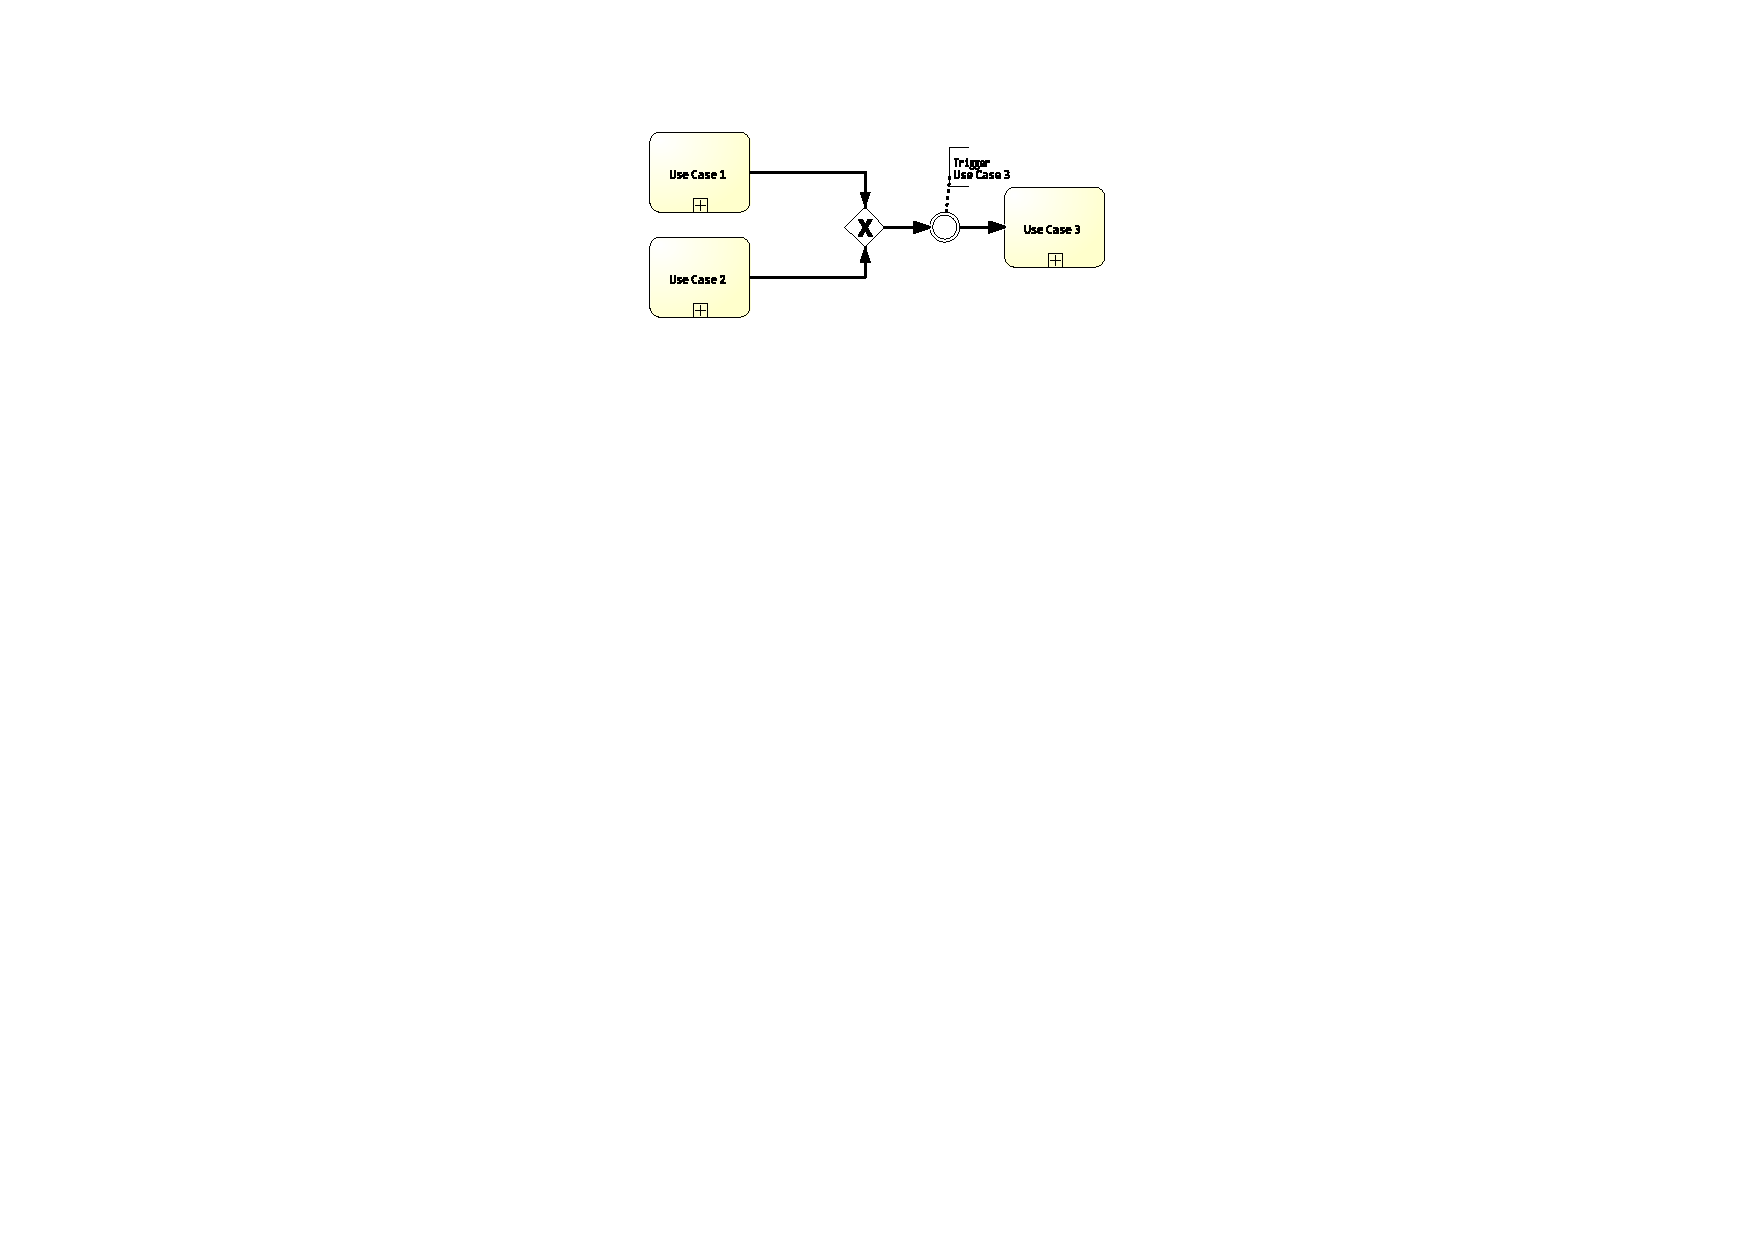
\includegraphics[width=0.9\textwidth, trim={11cm 15cm 12cm 2cm}]{img/JoinBPMNpostcondition.pdf} % first figure itself
		\caption{Join multiple BPMN processes on same postconditions}
		\label{fig:JoinBPMNPostcondition} %11cm 14cm 18cm 1cm
	\end{minipage}\hfill
	\begin{minipage}{0.45\textwidth}
		\centering
		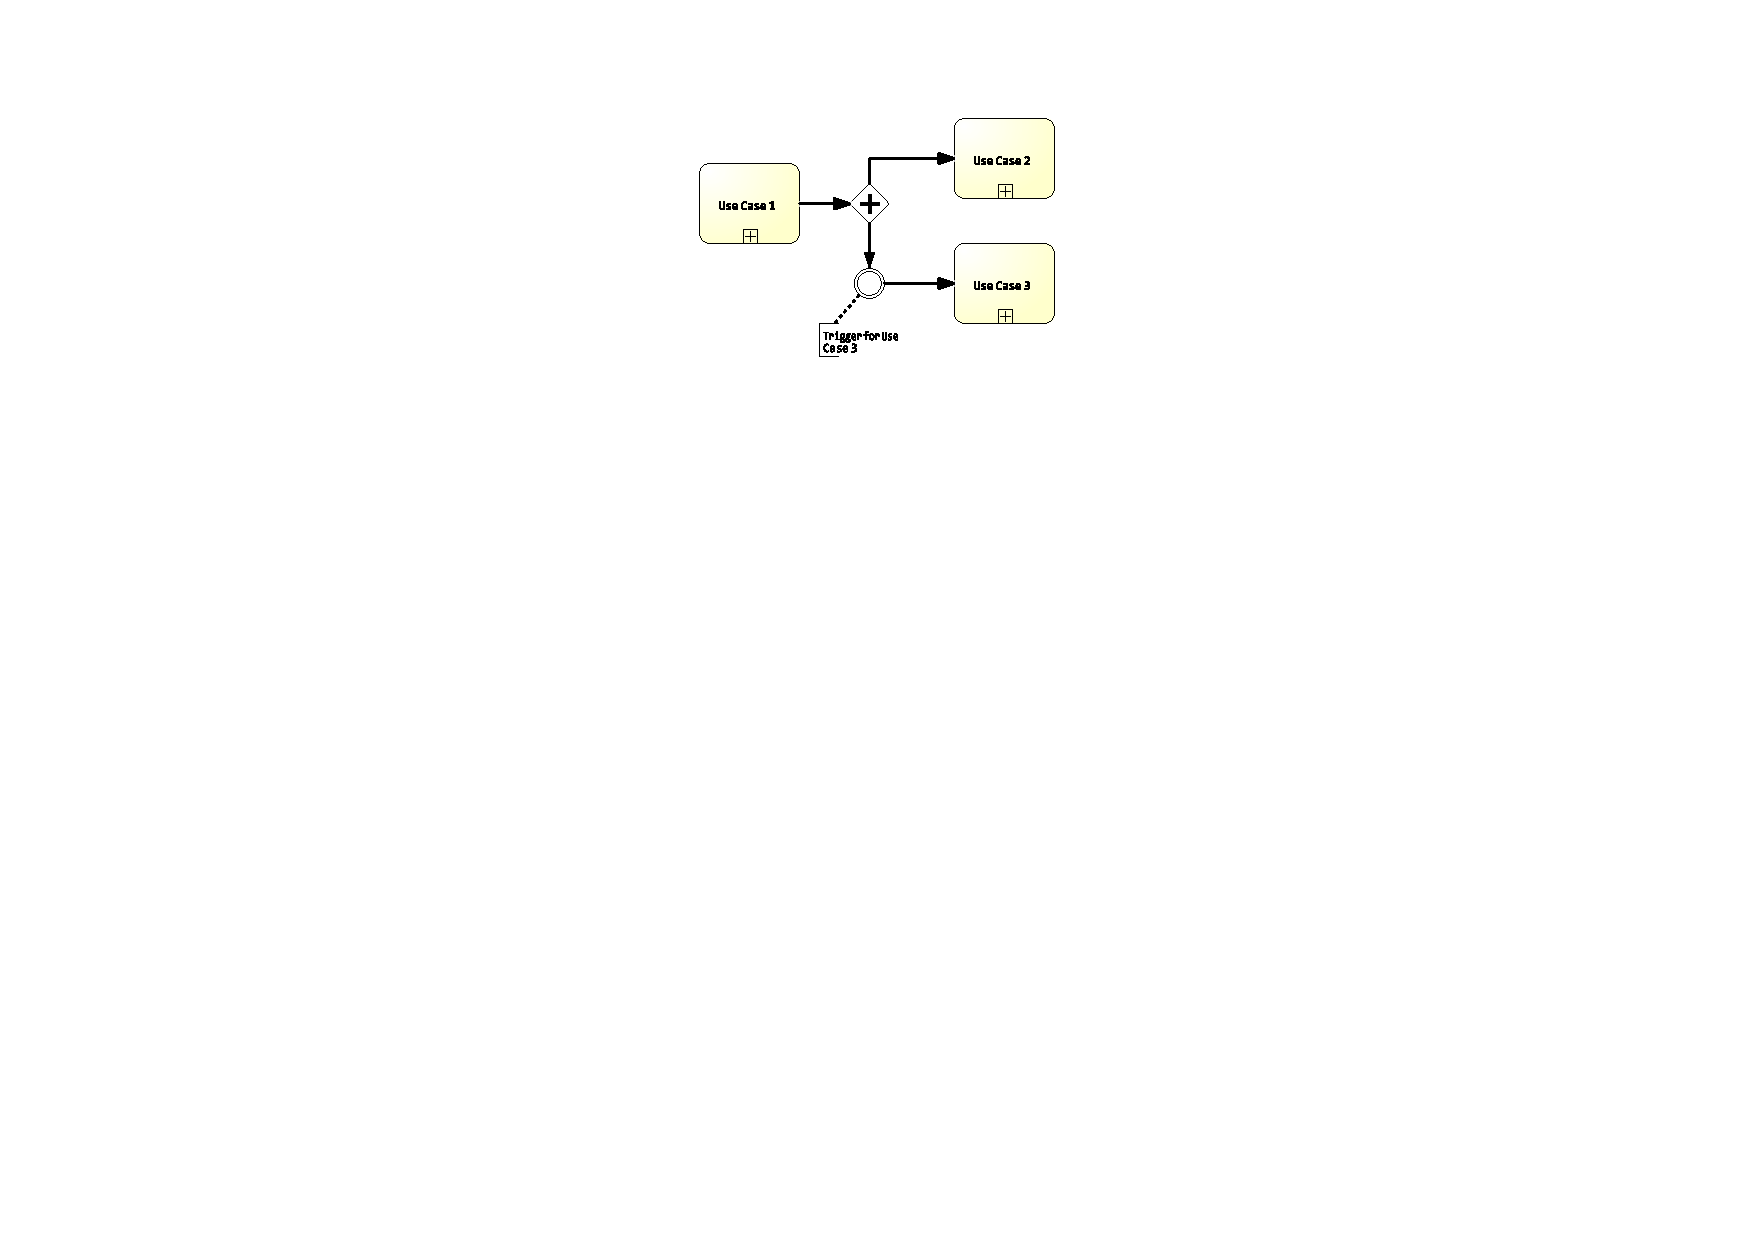
\includegraphics[width=0.9\textwidth, trim={11cm 15cm 12cm 2cm}]{img/JoinBPMNPrecondition} % second figure itself
		\caption{Join multiple BPMN processes on same preconditions or triggers}
		\label{fig:JoinBPMNPrecondition}
	\end{minipage}
\end{figure}

\noindent
If several use cases have the same preconditions or triggers and therefore use the same postcondition (Fig.\ref{fig:JoinBPMNPrecondition}), join them by introducing a Parallel Gateway and split the control flow. Notice, that the use cases in Fig.\ref{fig:JoinBPMNPostcondition} and Fig.\ref{fig:JoinBPMNPrecondition} are only displayed as collapsed subprocess for the sake of clarity. \\
Second to last, the resulting data associations and objects are refactored. Duplicate data objects that arose from joining two processes need to be eliminated. For each set of duplicate data objects, remove all but one and reconnect the existing data associations arcs to the remaining object. \\ 
Finally, all business models need to be refactored. Whereas the prior steps are very algorithmic and follow a predefined concept, this step includes non-trivial work. Due to the fact that use cases are given in natural language, one has to identify synonymous data objects, steps, triggers, post- and preconditions. Moreover, a step in an use case may include two activities and has to be split up. For example, given these two steps from two different use cases:
\begin{itemize}
	\item \textit{The Store Manager changes the sales price of the Stock Item and commits the change by pressing enter}
	\item \textit{The sale information is sent to the Inventory in order to update the Stock}
\end{itemize}
Both steps update the same data object, which is the \textit{Stock Item}, although the second step refers to the object as \textit{Stock}. The activity in both cases can be described as \textit{Update inventory}. Furthermore, step one contains two activities and needs to be split in \textit{Change Price} and \textit{Update Inventory}.



\subsection{Limitations and Drawbacks of the Transformation}
In the previous section, a method to transform use cases in a set of BPMN models is introduced, as the running example only provides system specifications in form of detailed use cases (cf.\ref{ch:CoCoME}). However, this transformation requires a non-trivial refactoring process. \\
In regard to data objects, it is obvious that multiple appearances of the same object (in different shaping) in a process devastate the resulting data flow. Hence, it is necessary to eliminate synonyms to ensure an unadulterated outcome.\\
Speaking of tasks, it is indispensable to identify common tasks among all use cases and hence, the resulting business processes to create the structural relationship between them. If not, the tasks would be arranged in a circle-like order and the resulting clusters would correspond to the single business processes. Structural dependencies between processes like using the same functionalities would disappear.\\
For this reasons, the refactoring process has to be conducted 
conscientiously. If this is not the case or synonyms etc. are not identified, the results of the approach might not be satisfactory.




\section{Extract Control Flow}
\label{sec:Solution:ExtractControlFlow}
In the course of the process, activities of the business processes are clustered based on their structural dependency which is extracted from the control flow. Activities (tasks) in business processes play the role of operations in microservices, representing the functionality a service is able to offer. During the process of microservice identification, it is desired to cluster highly cohesive functionality into one microservice. To achieve this, one must first extract the structural  dependencies between activities in business processes. \\
The extraction process itself is trivial, as the business process language BPMN was designed to illustrate the control flow between activities (cf. Sec.\ref{sec:PrepApproach:BPMN}). Mainly inspired by the work of M. Amiri in \textit{Object-aware Identification of Microservices} \cite{ObjectAwareAmiri}, we propose a straightforward technique to separate the control flow information from BPMN 2.0 models:\\
All that has to be done is to delete the Data Objects and the accompanying associations. The remaining diagram visualizes the control flow, including activities and their control flow dependencies. Further information can be extracted in various ways. For instance, counting the amount of tasks between a pair of activities provides information about their structural dependency. The control flow has to be extracted for each BPMN model that was specified in the previous step.
 \section{Create a weighted Graph using Control Flow}
 \label{sec:Solution:CreateGraphControl}
 In section \ref{sec:Solution:ExtractControlFlow}, the control flow is extracted from several BPMN models that represent the entire system.
 The visualization of the control flow information as a single graph enables to identify clusters of highly cohesive functionality among all BPMN models, thus among the entire system. 
 Therefore, we build a directed graph G whose vertices represent the tasks/activities in the BPMN models. Duplicate vertices are not allowed. Hence, activities that occur several times in different BPMN models are only represented once in the graph.
 The edges correspond to the control flow arcs: a pair of activities is connected if there is a direct edge in the business processes or if there is a path between them that contains only gateways. This decision is based on the heuristic, that two activities are more likely to be in the same microservice, if they are directly connected in a business process. \\
 Speaking of the weights, we decide to assign a value of 1 to each edge, notwithstanding of the nature of the connection, which is i) directly connected ii) connected via parallel gateway iii) connected via XOR gateway. Regarding the first and the second case, it is motivated by the fact that activities connected by a parallel gateway and activities that are directly connected are always executed during control flow execution.
 In regard of the third case, one can argue that the probability of a condition influences the weight of a connection. For instance, a task has two subsequent tasks that are connected through an exclusive OR gateway and conditional flows. One of the tasks, the "main task", is more likely to be the successor as the alternative. Hence, the edges need a different weight. However, the information regarding the probability is usually not available and specified in business processes. Further, different weighting raises the question of the value determination. With this in mind, the generalization of all types of connections (using a weight of 1 for all edges) seems to be an appropriate solution. \\
 In the case of duplicated control flow dependencies due to several BPMN models, the weights are summed up as a pair of connected tasks that occur in multiple models indicates a stronger cohesion. As a result, the edge in the graph that connects the tasks in questions receives a greater weight (corresponding to the number of occurrences).\\
 Fig.\ref{fig:controlFlow} shows an exemplary BPMN process whose object-related information has already been deleted (cf. Sec.\ref{sec:Solution:ExtractControlFlow}). As explained in this section, the control flow information given in this BPMN model is used to create a weighted graph. The corresponding graph is illustrated in Fig.\ref{fig:controlFlowGraph}. 
 
 
 \begin{figure}[h!]
 	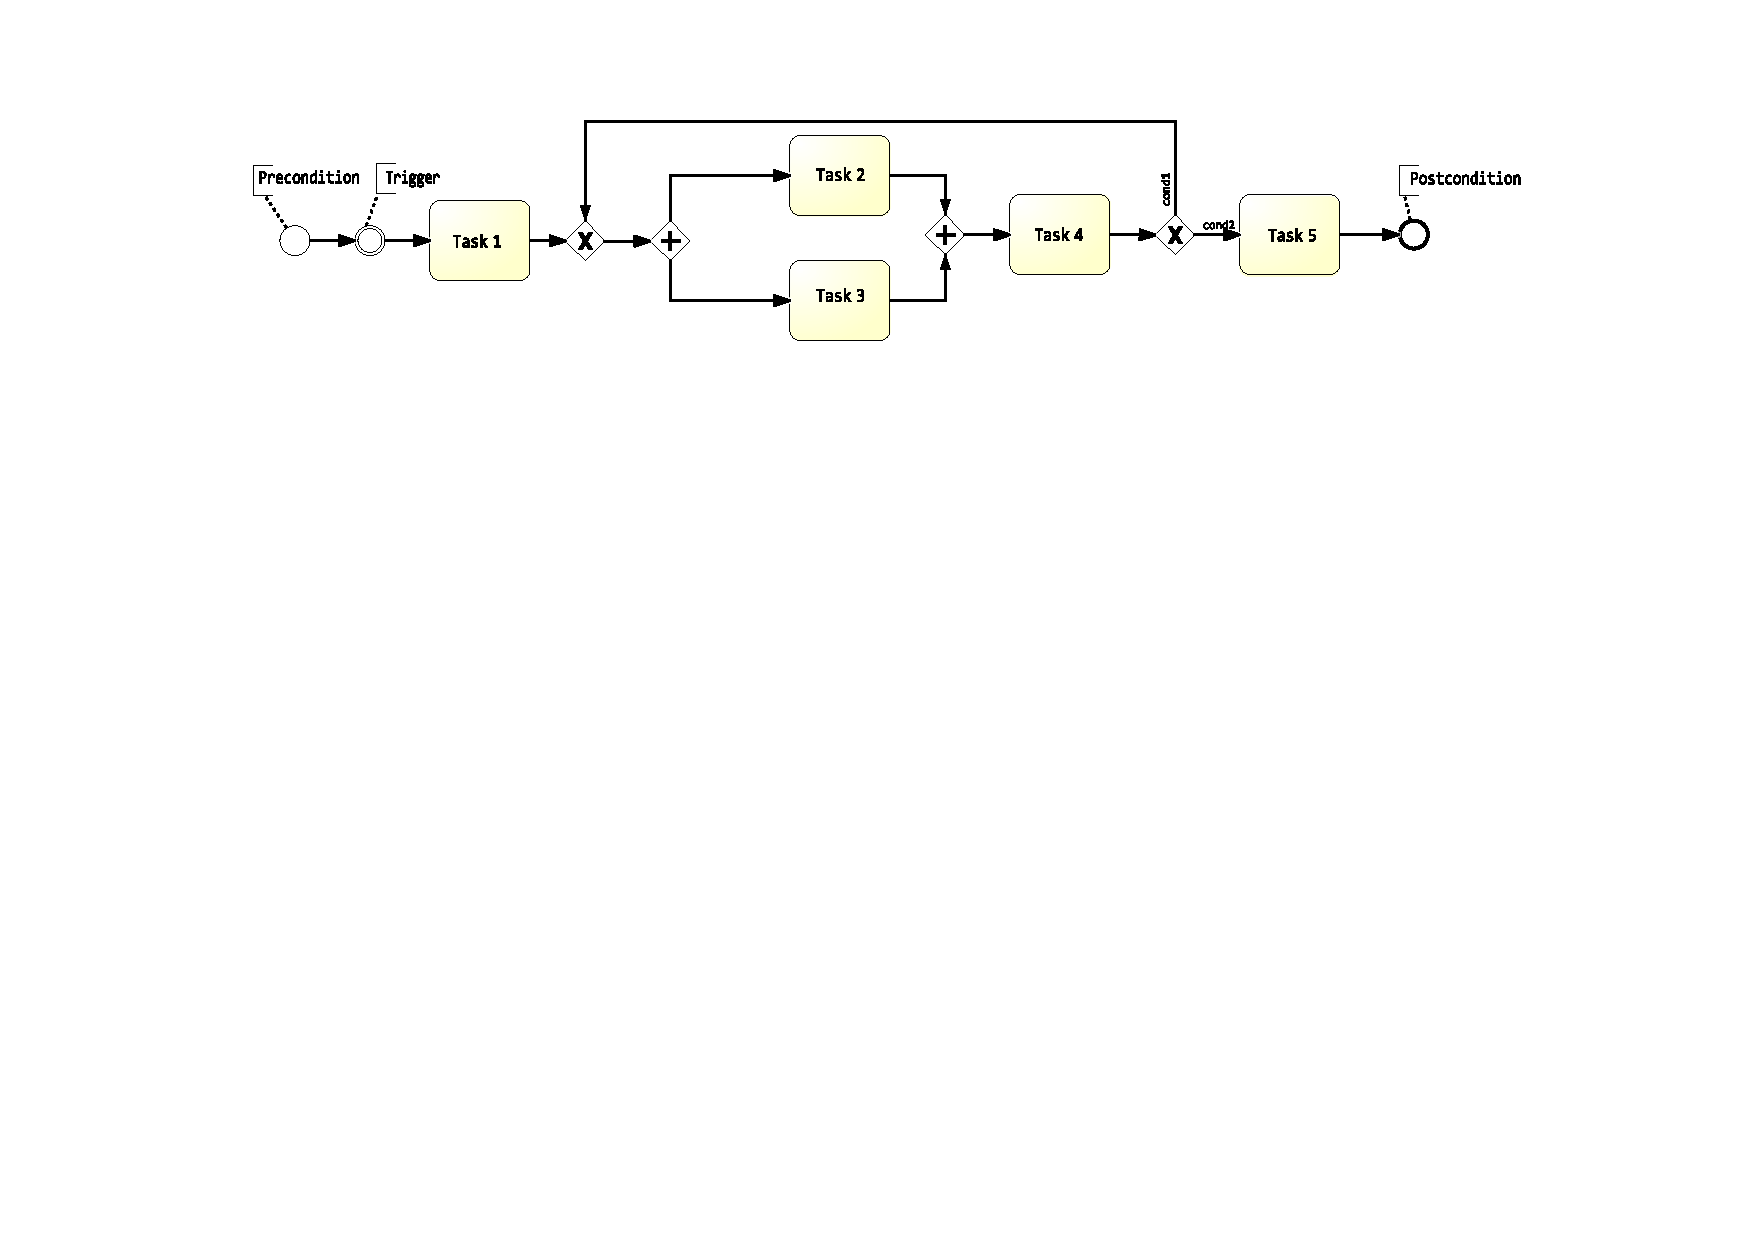
\includegraphics[width=\textwidth, trim={4.5cm 14cm 4.0cm 1.5cm}]{img/ControlFlowExample.pdf}
 	\caption{An exemplary BPMN model illustrating the control flow only  }
 	\label{fig:controlFlow}
 \end{figure}
 %"l, b, r, t"
 \begin{figure}[h!]
 	\centering
 	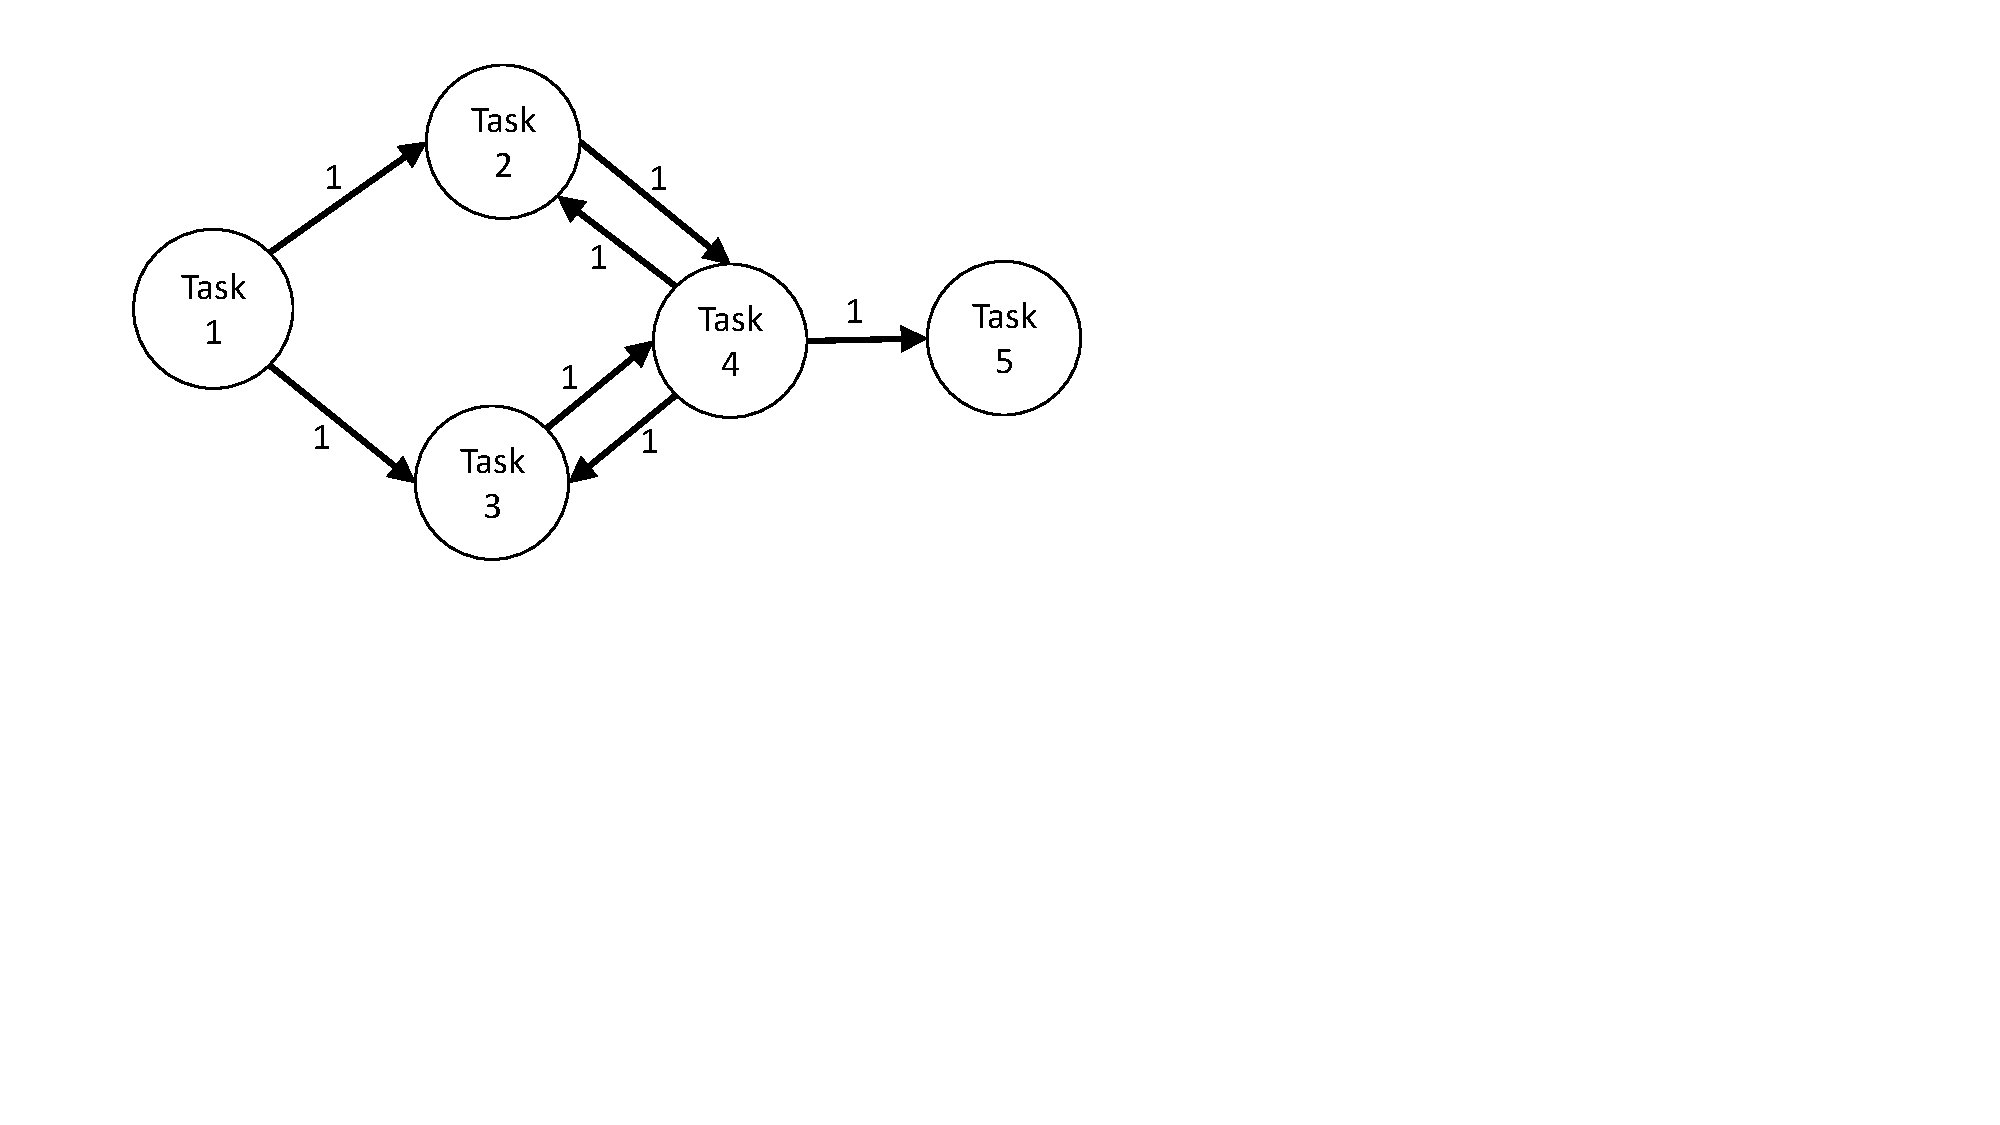
\includegraphics[width=12cm, trim={1.5cm 9.0cm 13.0cm 0cm}]{img/ControlFlowGraph.pdf}
 	\caption{Weighted graph using Control Flow Dependencies}
 	\label{fig:controlFlowGraph}
 \end{figure}
 
 

\pagebreak

\section{Extract Data Flow}
\label{sec:Solution:ExtractDataFlow}
Besides the structural dependencies of activities, data object access plays a significant role in the definition of microservices. As depicted in the background chapter \ref{ch:background}, microservice generally administer their own database with the data entities that belong to the bounded context of the service. Usually, data needs to be shared among services which raises the question where to place a shared data object. However, sharing data among microservices is expensive because it includes network communication instead of inter process communication. It is therefore desirable to reduce the communication between services by distributing data objects into the same microservice if they are accessed together.  
Like the previous section, we propose to use clustering based on data flow to identify highly cohesive but loosely coupled set of data object clusters. \\
Usually, data flows are represented using specific notations of Data Flow Diagrams (DFD), i.e. a notation proposed by E.Yourdon \cite{YourdonDFD}. For simplicity's sake, we relinquish to introduce another model notation and use the BPMN symbols instead. \\
When BPMN 2.0 was introduced, the language was extended by the ability to represent data objects that are consumed and/or produced by the activities. Despite the fact that BPMN is still a language to illustrate the control flow of business processes, the 2.0 extension provides the possibility to visualize an approximated data flow based on the data needs and writes of each activity. The approximation is necessary due to the capability of BPMN to express the data needs and the data results of single activities only, whereas the data flow describes the flow of data in a process. By way of Fig.\ref{fig:restoreDataFlow}, \textit{Step 1} reads \textit{Data Object 1} and writes \textit{Data Object 2}. Despite the information about the data reads and writes of \textit{Step 1}, it is not possible to determine without further knowledge, if any information of \textit{Data Object 1} is used to write into \textit{Data Object 2}. Usually, this information has to be provided by system experts. \\

%"l, b, r, t"
\begin{figure}[h!]
	\centering
	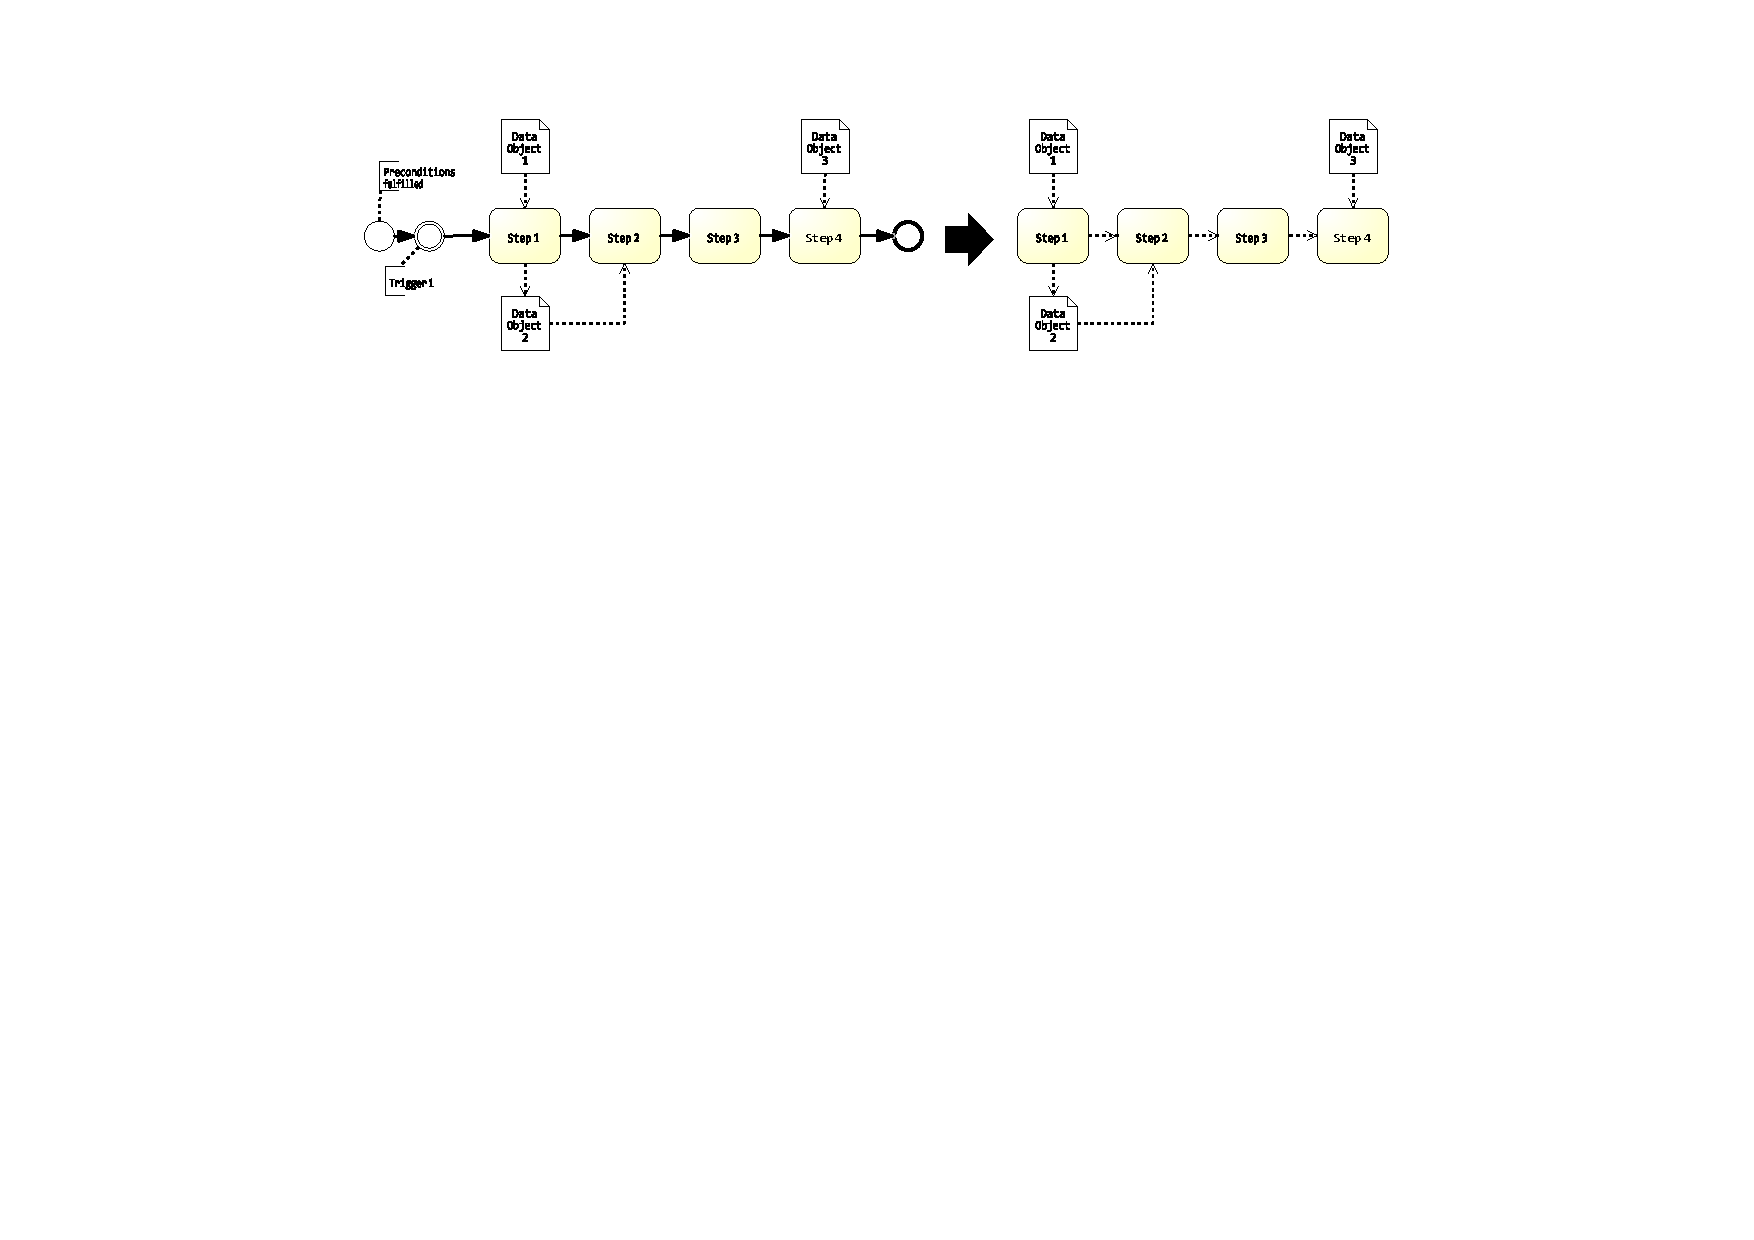
\includegraphics[width=\textwidth, trim={7.5cm 15cm 7cm 2cm}]{img/ExtractDFDRestore.pdf}
	\caption{Restore data flow connection}
	\label{fig:restoreDataFlow}
\end{figure}

\noindent
However, the approach presented in this thesis aims to reduce the required expertise and the additional information that is necessary during the execution. 
Hence, it is fundamental to approximate the data flow based on the data needs and writes of each activity. As in this case, the approximated data flow has to be extracted for each BPMN model. \\
First of all, control flow related parts like sequence flows arcs, gateways, events and triggers are deleted. The remaining parts are tasks, data objects and data associations. Now, the tasks are not connected to their previous neighbours, with which they might exchange data. In this case, data exchange is synonymous with the flow of data.
To re-establish the possible data flow, follow the previously deleted control flow and reconnect the tasks with data association arcs by applying the following rules:

\begin{itemize}
	\item Connect a pair of tasks if previously connected by a control flow arc and 
	if another data object access happens in the course of the control flow (cf. Fig\ref{fig:restoreDataFlow})
	\item Replace gates by using two data association arcs (cf. Fig.\ref{fig:splitDataFlow} and Fig.\ref{fig:mergeDataFlow}). 
	\item Remove the remaining tasks that are not connected by data association arcs (cf. Fig.\ref{fig:removeDataFlow})
	
\end{itemize}
The remaining Graph contains all relevant tasks, the data objects and data associations that indicate the flow of data.



\begin{figure}[h!]
	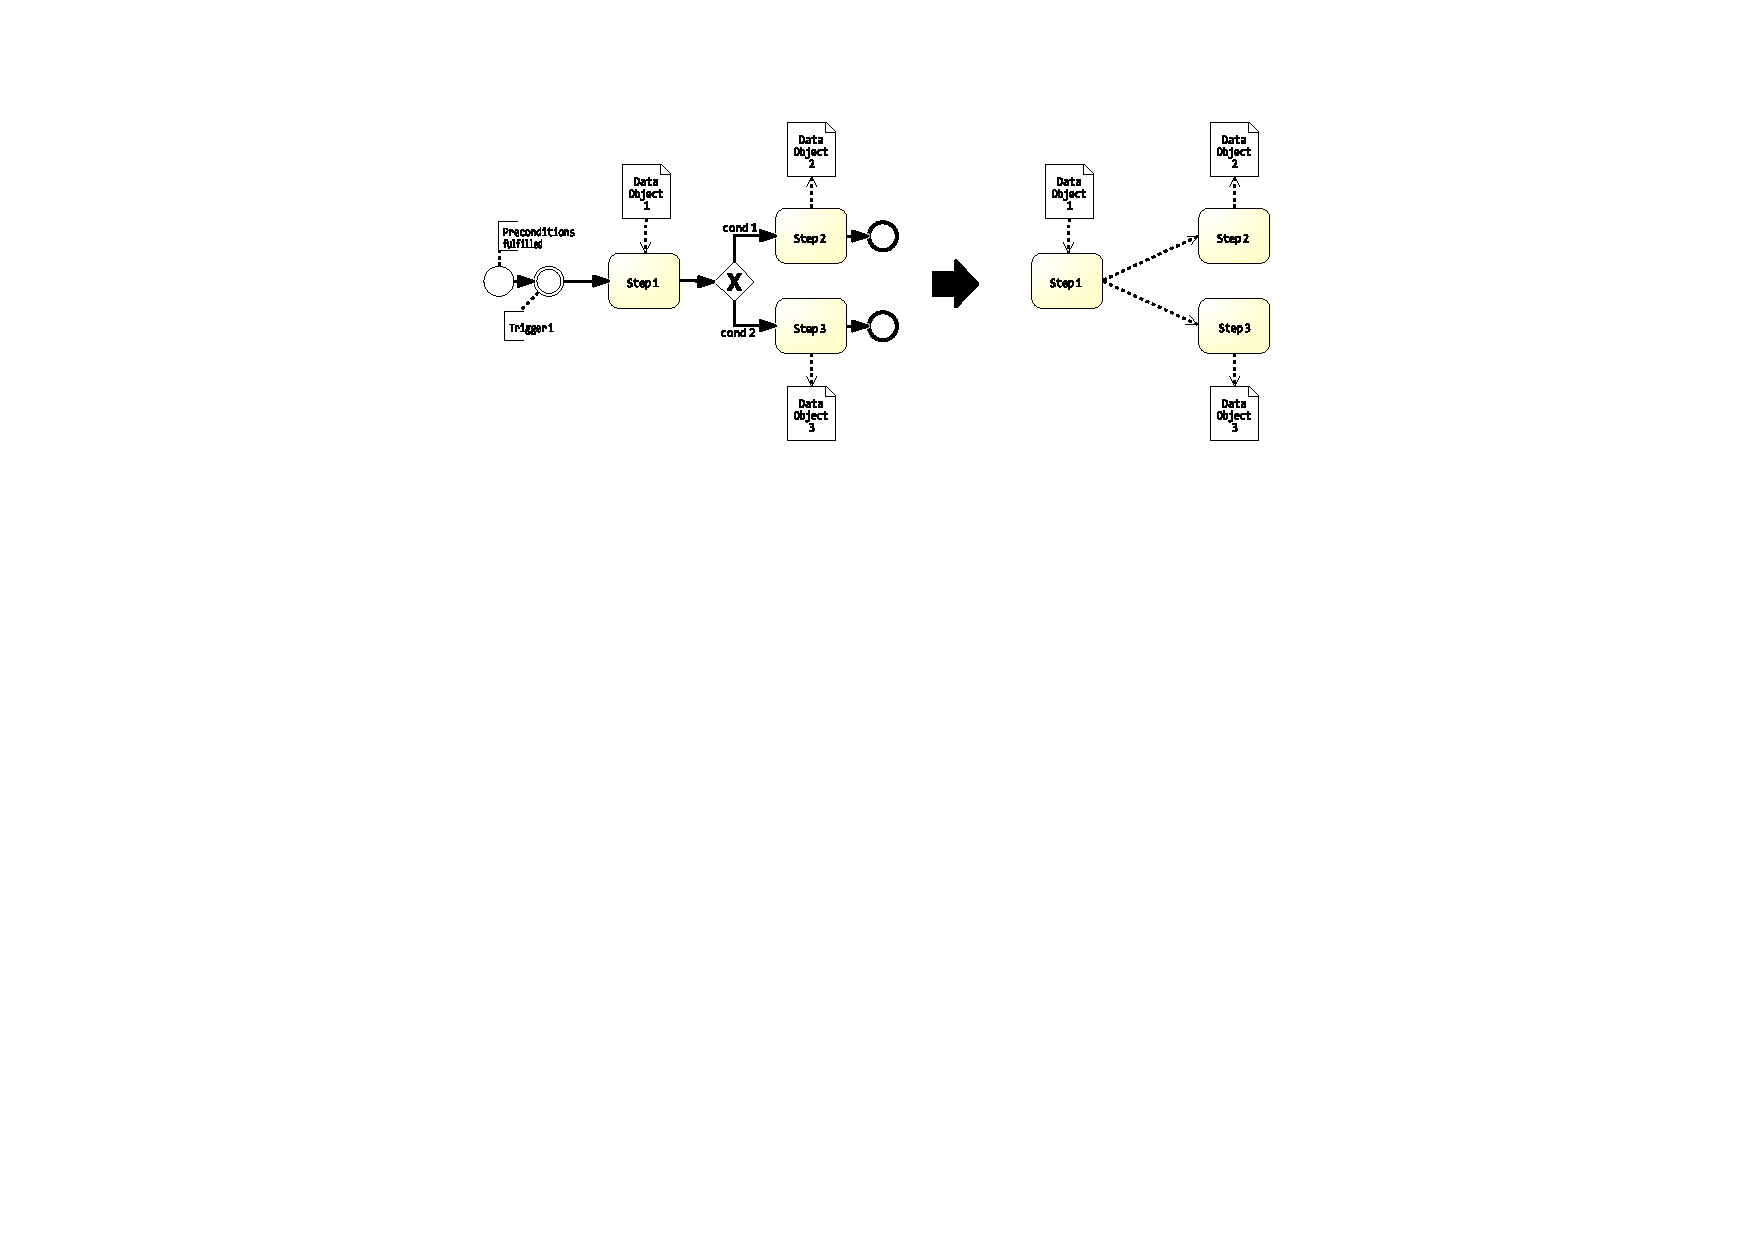
\includegraphics[width=13cm, trim={8.5cm 13.8cm 8.5cm 2.2cm}]{img/ExtractDFDGateWaySplit.pdf}
	\caption{Split data flow connection}
	\label{fig:splitDataFlow}
\end{figure}

\begin{figure}[h!]
	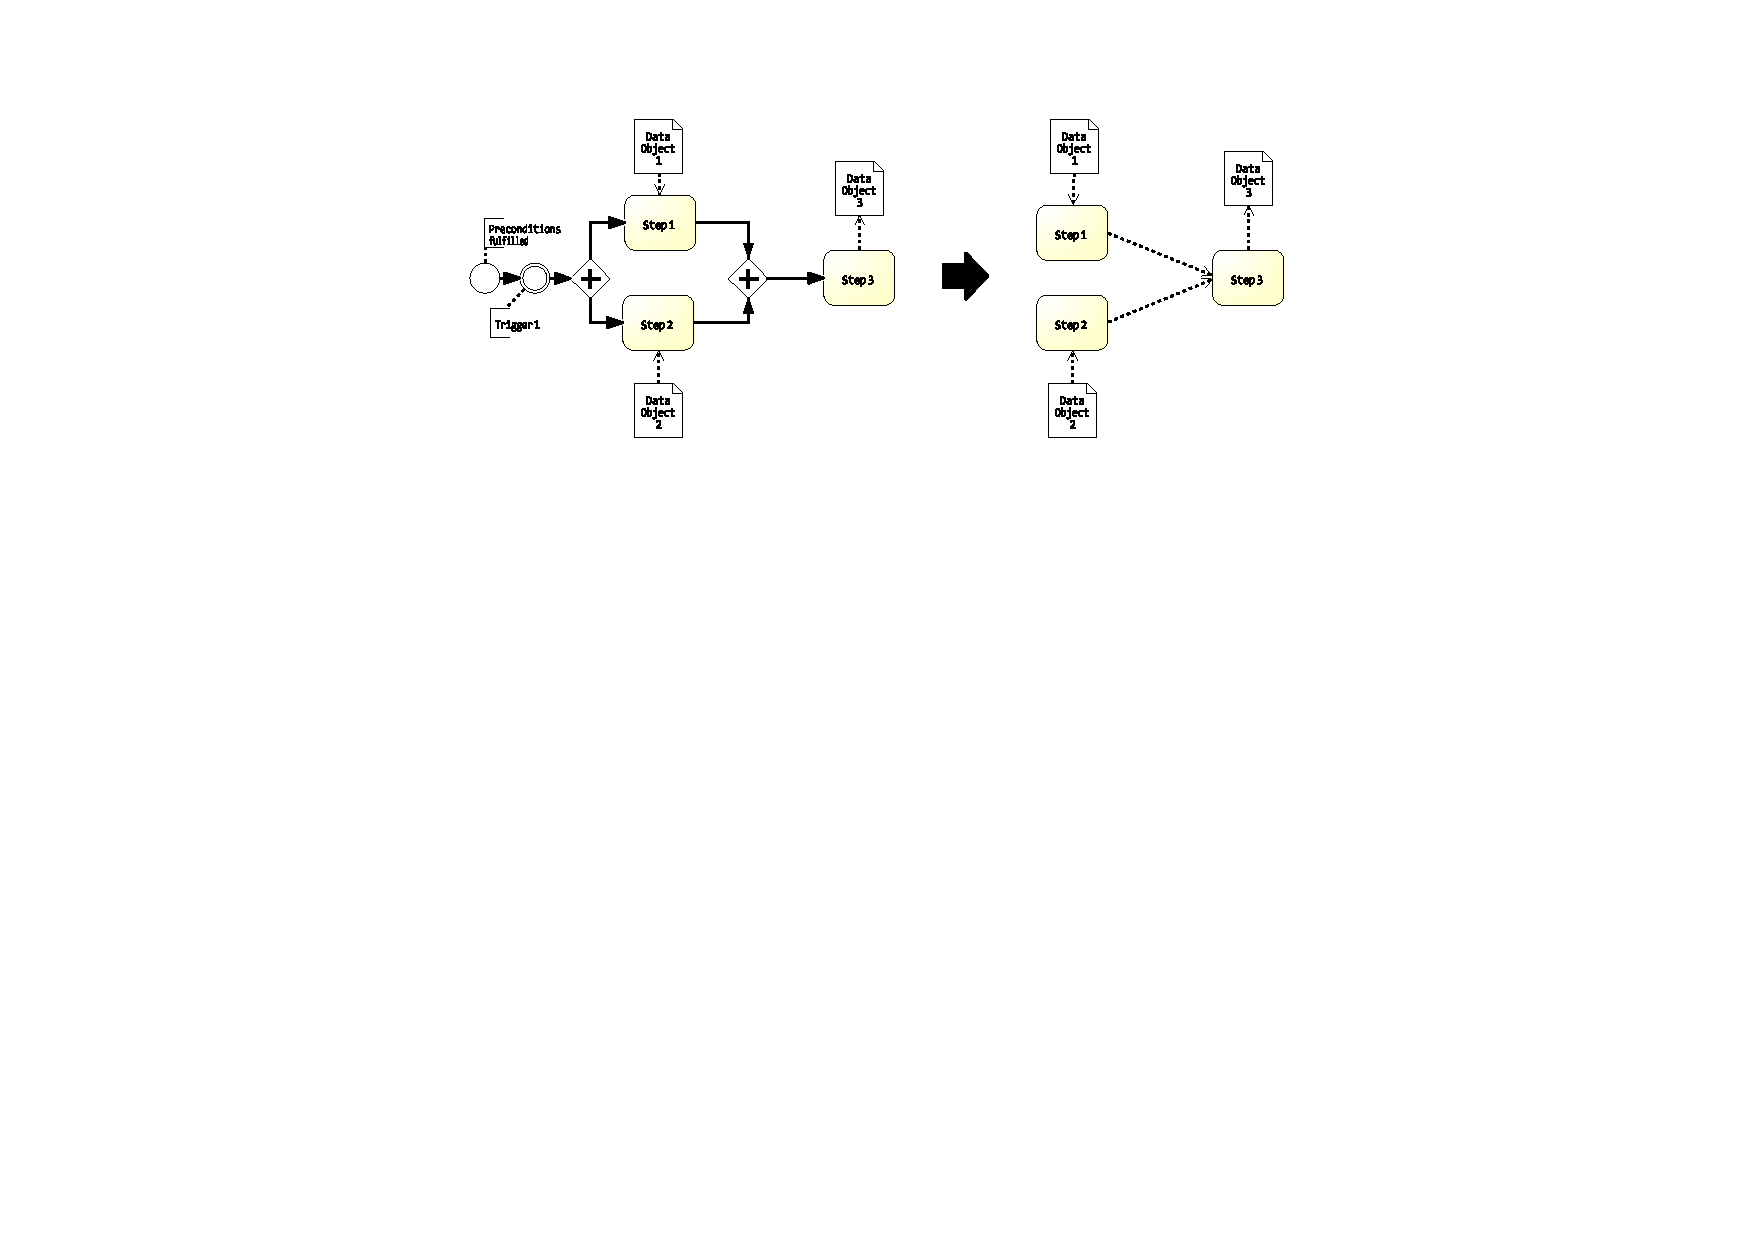
\includegraphics[width=14cm, trim={8.5cm 13.5cm 8.5cm 2.0cm}]{img/ExtractDFDGateWayMerge.pdf}
	\caption{Merge data flow connection}
	\label{fig:mergeDataFlow}
\end{figure}

\begin{figure}[h!]
	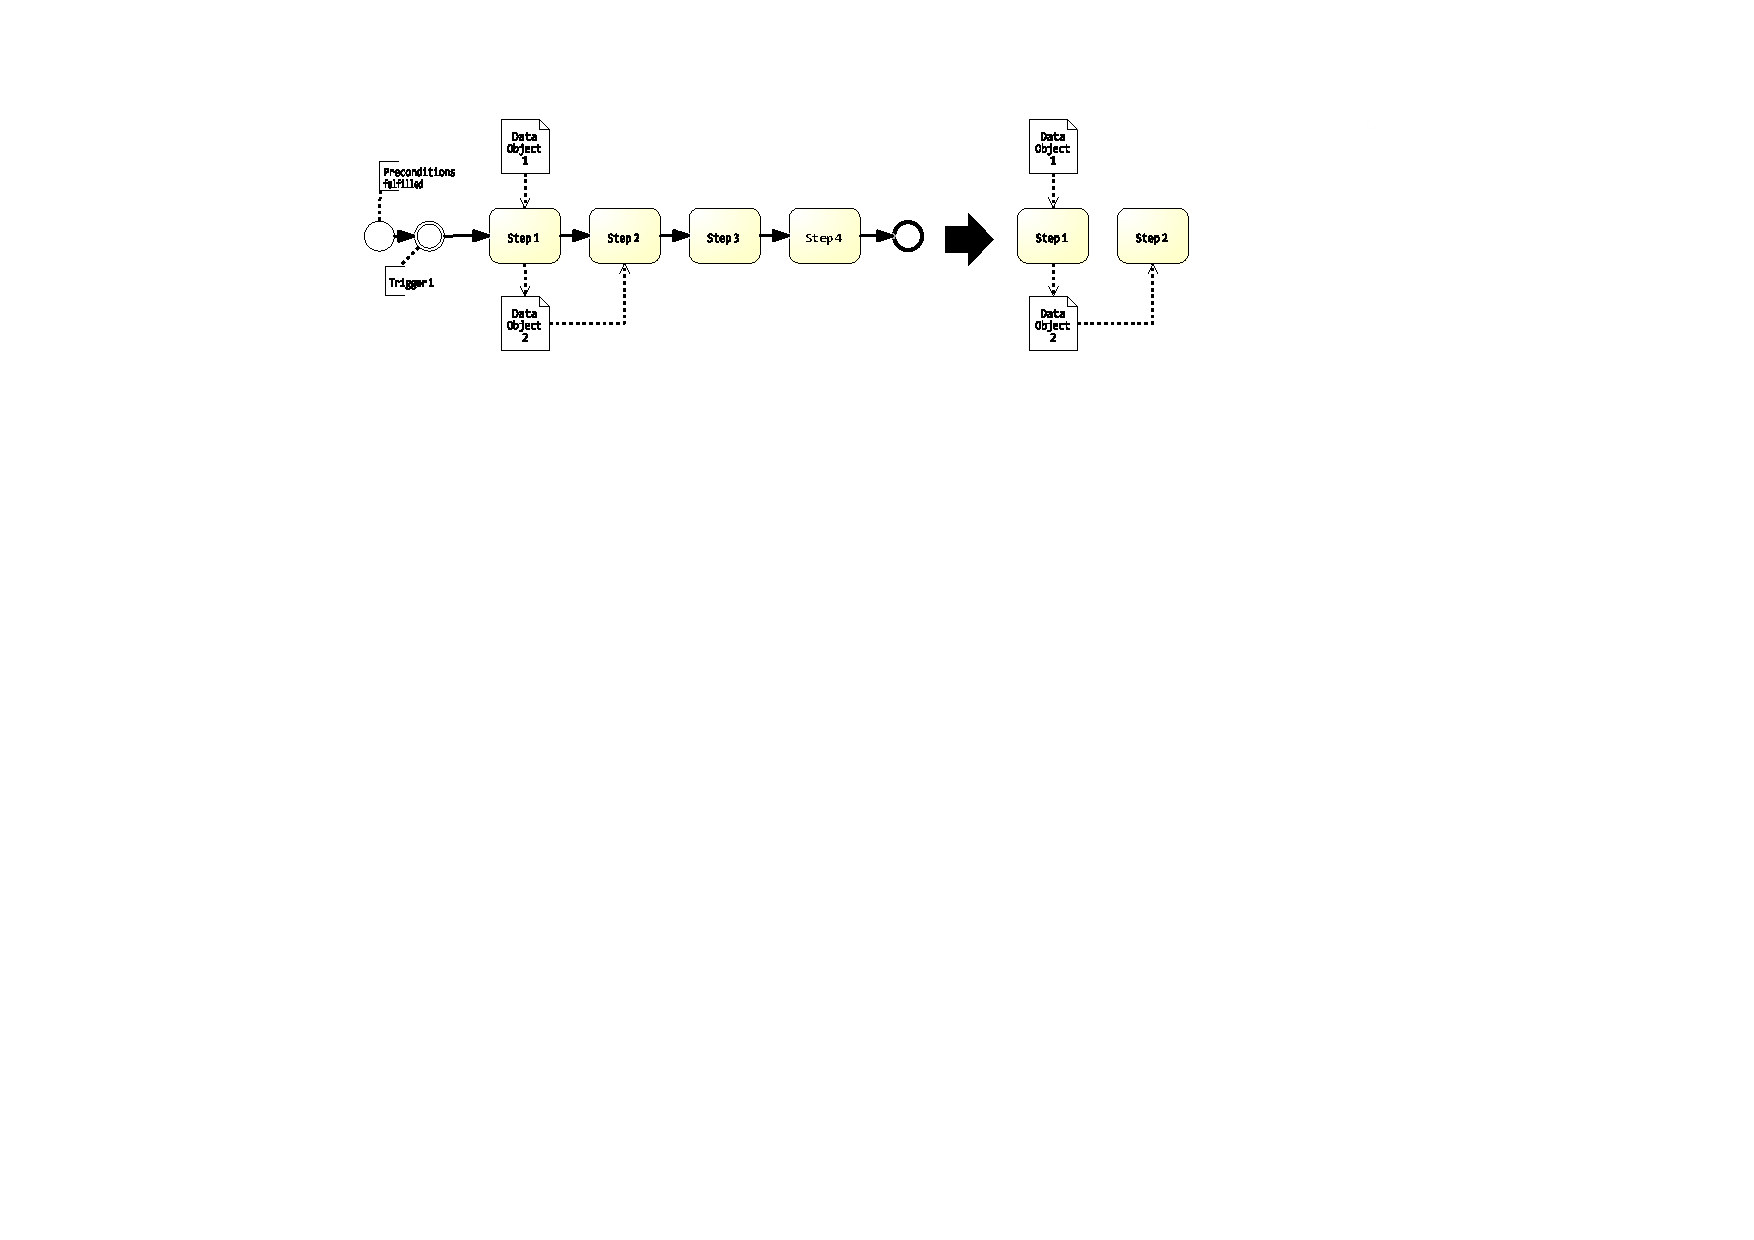
\includegraphics[width=\textwidth, trim={7.5cm 15.3cm 8.5cm 1.5cm}]{img/ExtractDFDRemove.pdf}
	\caption{Remove unnecessary tasks}
	\label{fig:removeDataFlow}
\end{figure}



\pagebreak







\pagebreak



\section{Create a weighted Graph using Data Flow}
\label{sec:Solution:CreateGraphData}
To identify highly cohesive data object clusters, the data flow information is visualized as a weighted graph, which is similar to the activity graph as described in the previous sections. In this case, the vertices of a Graph G represent the data objects in the BPMN models. Like the activity graph, duplicated vertices are not allowed. Each data object is only represented once in the graph. The edges illustrate the data object dependencies extracted from the data flow. \\
Such dependencies are: i) data objects read by the same task ii) a data object value that is used when writing to (or creating) another data object. \\
Speaking of the first dependency, it is obvious that data which is read by the same task is more likely to be partitioned into the same service. Otherwise, the execution of a task would always cause at least one expensive intra-service call.
Therefore, a pair of data objects represented by two vertices are to be connected by an edge in case they are both read by the same task.\\
The second dependency is based on a similar heuristic. There is a certain connection between two data objects, if information of one data object is used to update or create another one. Placing the information source into another microservice as the information destination would require an inevitable cross-service communication which is meant to be prevented. \\
To create a weighted graph based on data flow dependencies, it is necessary to take a closer look at the extracted data flow (cf. Sec.\ref{sec:Solution:ExtractDataFlow}). It is noticeable that it requires additional information to decide whether two data objects have one of the proposed connections. Fig.\ref{fig:dataFlowExample} represents an exemplary data flow diagram that was extracted from a BPMN process. In the following, we discuss different possibilities to gain the data object dependencies.


%"l, b, r, t"
\begin{figure}[h!]
	\centering
	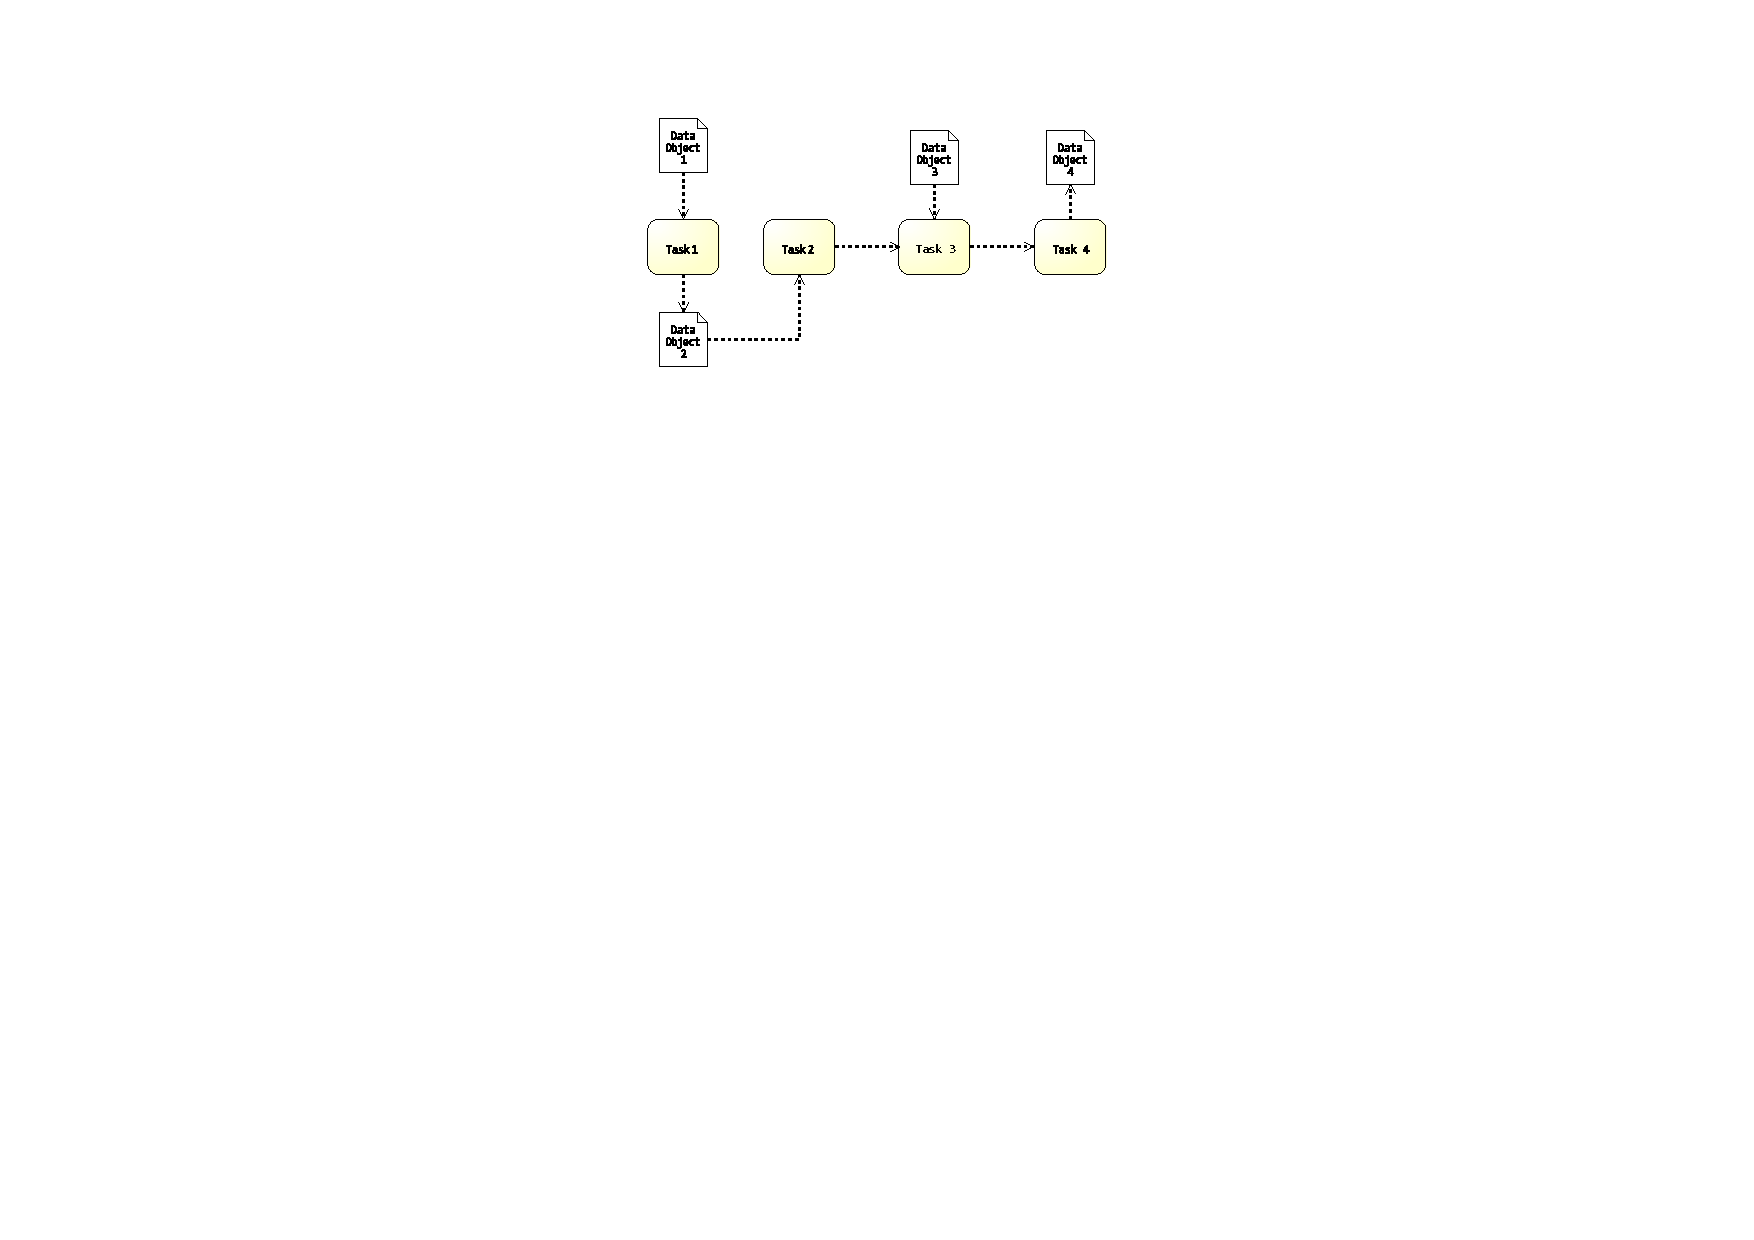
\includegraphics[width=12cm, trim={10cm 14.5cm 10cm 2cm}]{img/DataFlowExample.pdf}
	\caption{Data Flow Diagram extracted from BPMN process}
	\label{fig:dataFlowExample}
\end{figure}

\noindent
Information of one data object can flow into another one. That is the case, if a data object is updated or created using information of another data object which was read beforehand. 
For instance, \textit{Task 3} processes information of \textit{Data Object 3}, passes it to \textit{Task 4}, which uses the information of the data object to update \textit{Data Object 4}. Consequently, \textit{Data Object 3 \& 4} should be connected by an edge in the resulting data object graph. Yet, another possibility is that \textit{Task 3} only reads \textit{Data Object 3} and displays some information to the user. Further, \textit{Task 4} only processes user input to update \textit{Data Object 4}. Hence, \textit{Data Object 3 \& 4} are not to be connected by an edge, as there is no information flow in between. \\
The same line of reasoning can be applied to \textit{Task 1}: Information of \textit{Data Object 1} may or may not flow into \textit{Data Object 2}, although both data accesses are executed by the same task. As a final point, the information of several data objects may flow into another one. For example, \textit{Data Object 2}, produced by \textit{Task 1} and \textit{Data Object 3}, read by \textit{Task 3}, may be used to create \textit{Data Object 4}. Given these points, identifying data object dependencies has to be estimated. The following possibilities are available to estimate the data dependencies:


\begin{itemize}
	\item Dependency between a pair of data objects, only if both data objects are read and written by the same task.
	\item Dependency between a pair of data objects, if \textit{n} tasks\footnote{n $\in [0..]$, where 0 represents neighbouring tasks} are in between a task that reads the first data object and another task that writes into the other data object\footnote{Following the Data Flow Arcs when counting}.
	

	
	\item Use additional information to determine the actual data flow dependencies
\end{itemize}
\noindent
The dependencies are expressed by connecting the vertices in question (which represent the data objects) with a weighted edge. 
Obviously, the third possibility is the most accurate one. The identified data object dependencies correspond to the reality. Though, one of the thesis' goals is to reduce human involvement to a minimum, so that the approach is able to run without further user interaction. Consequently, this possibility is discarded. \\
Regarding the first option, data object dependencies are frequently underestimated, as no information flow from one task to another is discerned. For this reason, option one is also discarded. \\
With this in mind, the second option seems to be the most appropriate one to determine the data flow dependencies based on the data flow graph. Still, the number \textit{n} has to be defined. Having \textit{n=0}, only data objects that are processed by neighbouring tasks are considered to share a dependency, therefore connected by an edge. This is reasonably similar to the control flow dependency, where only neighbouring tasks are connected by an edge as well. However, we empirically examined the data flow with \textit{n=0} and experienced an underestimation of the existing data flow dependencies. This is due to the fact that data processing and data storing is quite often distributed among several tasks. Fig.\ref{fig:ExampleDataProcessing} illustrates an example: 


%"l, b, r, t"
\begin{figure}[h!]
	\centering
	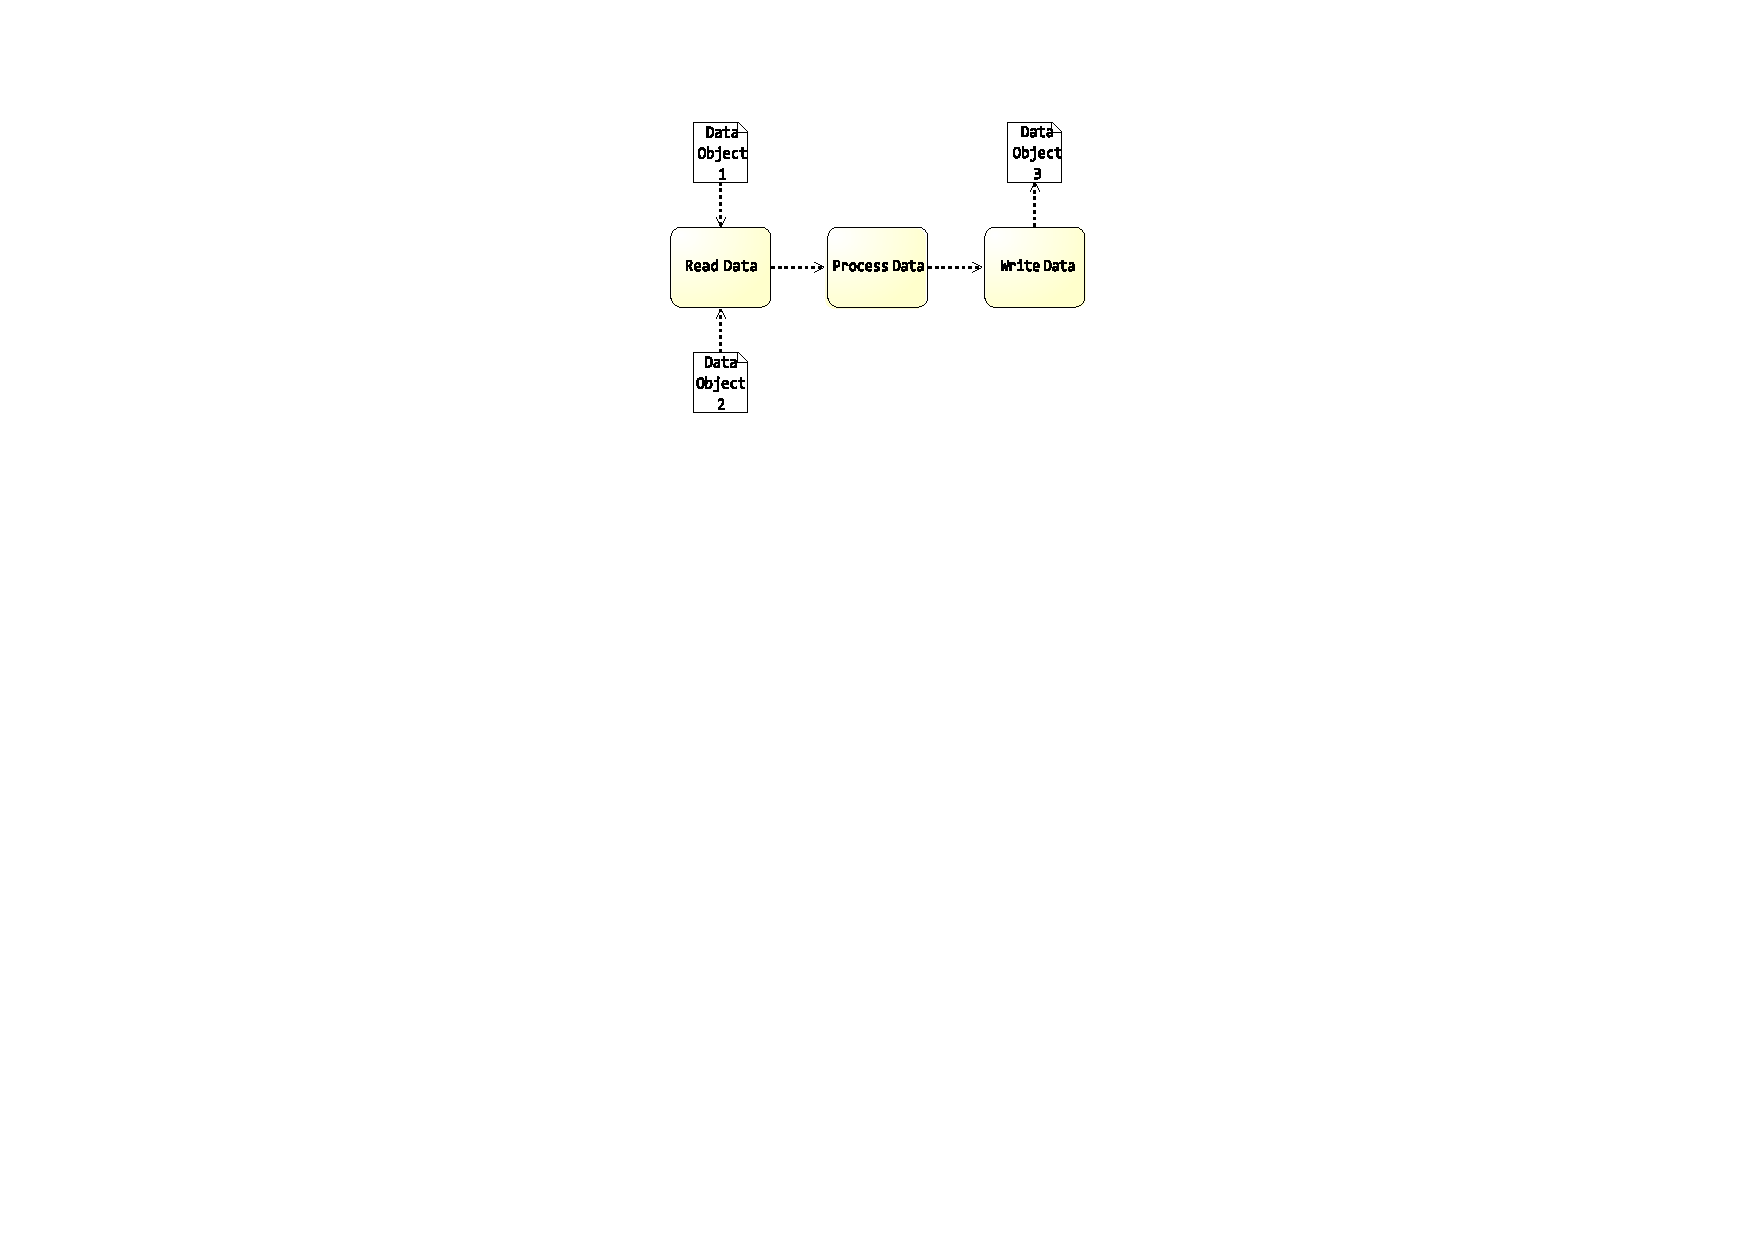
\includegraphics[width=9cm, trim={10cm 14.3cm 10cm 2.2cm}]{img/ProcessDataDFD.pdf}
	\caption{Data Flow Diagram to demonstrate data processing and data storing}
	\label{fig:ExampleDataProcessing}
\end{figure}

\noindent
Two data objects are read by the first task and passed to its neighbour, which is only in charge of processing it. Finally, the merged information is stored by a third task. To represent this common pattern of data processing, a value \textit{n>0} is required. \\
Nonetheless, reading and processing the data can be distributed among several tasks, depending on the granularity of the business processes. For instance, a more fine-granular business model divides the processing of \textit{Data Object 1} and \textit{Data Object 2} into two tasks, which still represents the same process.
Thus, determining the parameter \textit{n} highly depends on the granularity of the business processes. On the one hand, the value has to be big enough to cover data dependencies that are distributed among several tasks due to a more fine-grained process modelling. On the other hand, it should not be too big in order to prevent an overestimation of data dependencies due to data access which is executed by distant tasks. In our case, \textit{n=1} produced the best results. \\
Speaking of the weights, we decided to assign a weight of 1 to each each edge notwithstanding of the connection type, which again is i) two data objects are read by the same task ii) a data object value that is used when writing to another data object. Other approaches, like the one proposed by Amiri \cite{ObjectAwareAmiri} and Tyszberowicz \textit{et al.} \cite{FunctionalDecompositionHeinrich}, often differentiate between data reads and data writes, where the latter is generally weighted higher. However, the cross-service communication outweighs the difference between both data access types. In detail, a cross-service data read is generally much more time consuming compared to a inter-service write, due to the expensive network communication. Consequently, we propose to generalize data accesses by considering binary data dependencies only: two data objects are dependent according to the rules mentioned previously or they are not. 
In the case of duplicate data flow dependencies due to several tasks across various BPMN models that process the same data objects, the weights are summed up. This is motivated by the fact that multiple appearances of the same data object dependencies indicate a stronger cohesion.
Fig.\ref{fig:dataFlowGraph} illustrates the Graph that is produced when applying the approach to the data flow described in Fig.\ref{fig:dataFlowExample}.






%"l, b, r, t"
\begin{figure}[h!]
	\centering
	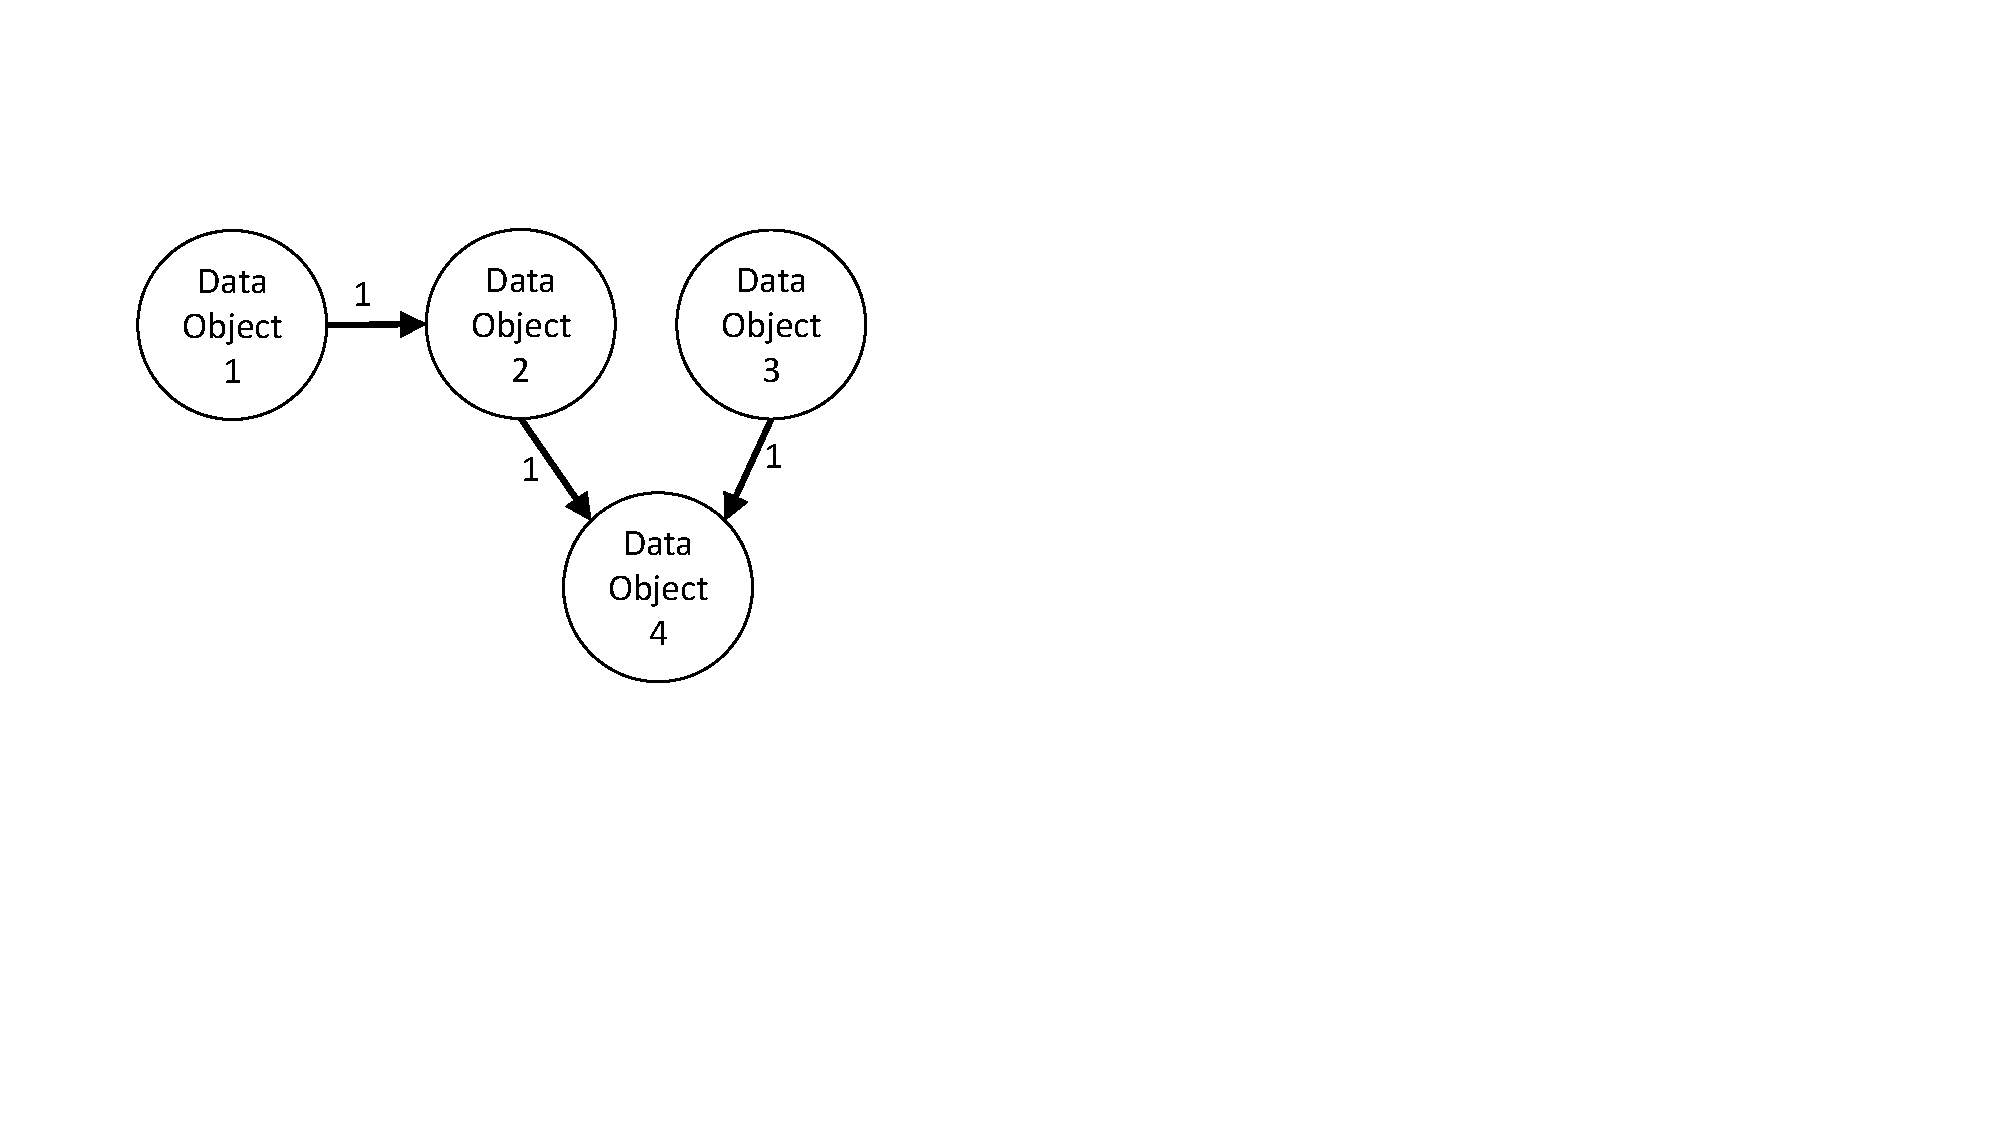
\includegraphics[width=10cm, trim={1.5cm 9.5cm 16.0cm 0cm}]{img/DataFlowGraph.pdf}
	\caption{Weighted graph using Control Flow Dependencies}
	\label{fig:dataFlowGraph}
\end{figure}


%"l, b, r, t" width=12cm, trim={1.5cm 7.5cm 13.0cm 2cm






\section{Identify Cluster}
\label{sec:Solution:IdentifyCluster}
The previous sections define strategies to represent the data flow and control flow dependencies as bi-directed weighted graphs. In this step of the identification process, the graphs are cut into disjunct set of nodes, called clusters. Common clustering techniques enable to identify sets of nodes with strong internal relationships and weak connections to the other clusters. The clustering is to be applied to both graphs equally, as they do not have any conceptual differences. At this point, it is important to emphasize that the elaboration of a clustering algorithm is beyond the scope of the paper. Therefore, we use existing tools for the visualization and identification of clusters. \\
In the course of this work, the first attempt to identify clusters involved the use of the graph visualization tool \textit{Gephi} \footnote{https://gephi.org/}. To layout the graph, the tool uses a force-directed algorithm based on gravity and repulsion called \textit{Force Atlas} \cite{gephi}. For the clustering, it uses a heuristic algorithm elaborated by Blondel \textit{et al.} to find "high modularity partitions of large graphs" \cite{modularity}. Whereas the activity clustering produced continuously constant results, the data object clustering did not. Despite using the same settings, the tool produced fair different sets of clusters when executing the algorithm. Obviously, the tool is not suitable for relatively small graphs as in the case of CoCoME.  \\
Upon further research, we choose a tool called \textit{Bunch}, which is a clustering tool that creates a graph decomposition by treating clustering as an optimization problem \cite{bunch}. \textit{Bunch} uses a genetic algorithm and a fitness function called \textit{Turbo-MQ} \cite{turbo-MQ}. In each iteration, the algorithm randomly picks \textit{K} clusters and calculates \textit{Turbo-MQ} to measure the fitness of the selected partition. In the next iteration, the algorithm tries to improve the fitness by making changes to the previous selected clusters. The algorithm stops, as soon as the overall fitness converges.\\

\pagebreak

\noindent
Mitchell \textit{et al.} defined the "modularization quality (=\textit{MQ}) measurement" \cite{turbo-MQ}, in such a way, that it rewards intra-cluster coupling while penalizing inter-cluster coupling:

\vspace{1cm}
\noindent
\begin{minipage}{.4\linewidth}
	
	\flushleft
	\begin{math}
	  Turbo-MQ = \sum_{i=1}^{k} CF_{i} 
	\end{math}
	

\end{minipage}%
\begin{minipage}{.5\linewidth}
	\flushleft
	\begin{math}
      CF_{i} = \begin{cases}
       0 & \mu_{i} = 0 \\
        \frac{\mu_{i}}{\mu_{i} + \epsilon_{i}}  & otherwise
      \end{cases}
  \end{math}


\end{minipage}
\vspace{1cm}

\noindent
The \textit{MQ} value of a partition with \textit{k} clusters is calculated by adding the \textit{Cluster Factor (CF)} of each cluster. $CF_{i}$ describes the normalized ratio between the total amount of internal edges $\mu_{i}$ and the amount of edges $\epsilon_{i}$ that originate in cluster \textit{i} and end in another cluster. The \textit{CF} value is between 0 (no internal edges) and 1 (no edge to another cluster), where larger values indicate a better quality of the partition. \\
Bunch requires the input graph in a simple textual form: The Graph is represented as list of edges, where each edge is described in a separate row by \textit{<start node>} \textit{<end node>} \textit{<weight>} (without the pointed brackets). The output is in the \textit{DOT} format \cite{DOT}, which is a powerful graph description language. To visualize the clustered graph, we use the open-source tool \textit{Graphviz} \footnote{https://www.graphviz.org/}.




\section{Match Cluster}
\label{sec:Solution:MatchCluster}
Having both sets of clusters, it is now necessary to match the activity clusters and the data clusters in a way that reduces the required inter-microservice communication. As a first step, it is necessary to count how many times an activity cluster accesses each data object cluster. When doing this, it is not desired to differentiate between read and write accesses. This decision is based on the same reasons as the weighting for the object dependencies is chosen (cf. Sec. \ref{sec:Solution:CreateGraphData}). The calculation of data access is a trivial task and only requires to examine the BPMN models one more time: For each activity that accesses a data object, identify the activity cluster the activity is located and the data object cluster the data is located. This is summarized for each pair of activity cluster and data cluster to obtain a relationship between the sets regarding the amount of accesses.\\
To process the obtained information, i.e. to match both sets of cluster, different approaches were elaborated during the course of the thesis:

\begin{itemize}
	\item Strongest relationship matching (data object cluster oriented)
	\item Strongest relationship matching (activity cluster oriented)
	\item Clustering on data access dependency
	\item White box approach: Split and/or merge cluster
\end{itemize}

\noindent
For the first three approaches, the respective clusters are considered from the black box point of view, as no closer look is taken into the actual clusters. Each cluster is represented as a node and connected by an undirected weighted edge, where the weights correspond to the respective amount of data accesses between the activity and the data cluster. Fig. \ref{fig:matchCluster} provides an example.\\

%"l, b, r, t"
\begin{figure}[h!]
	\centering
	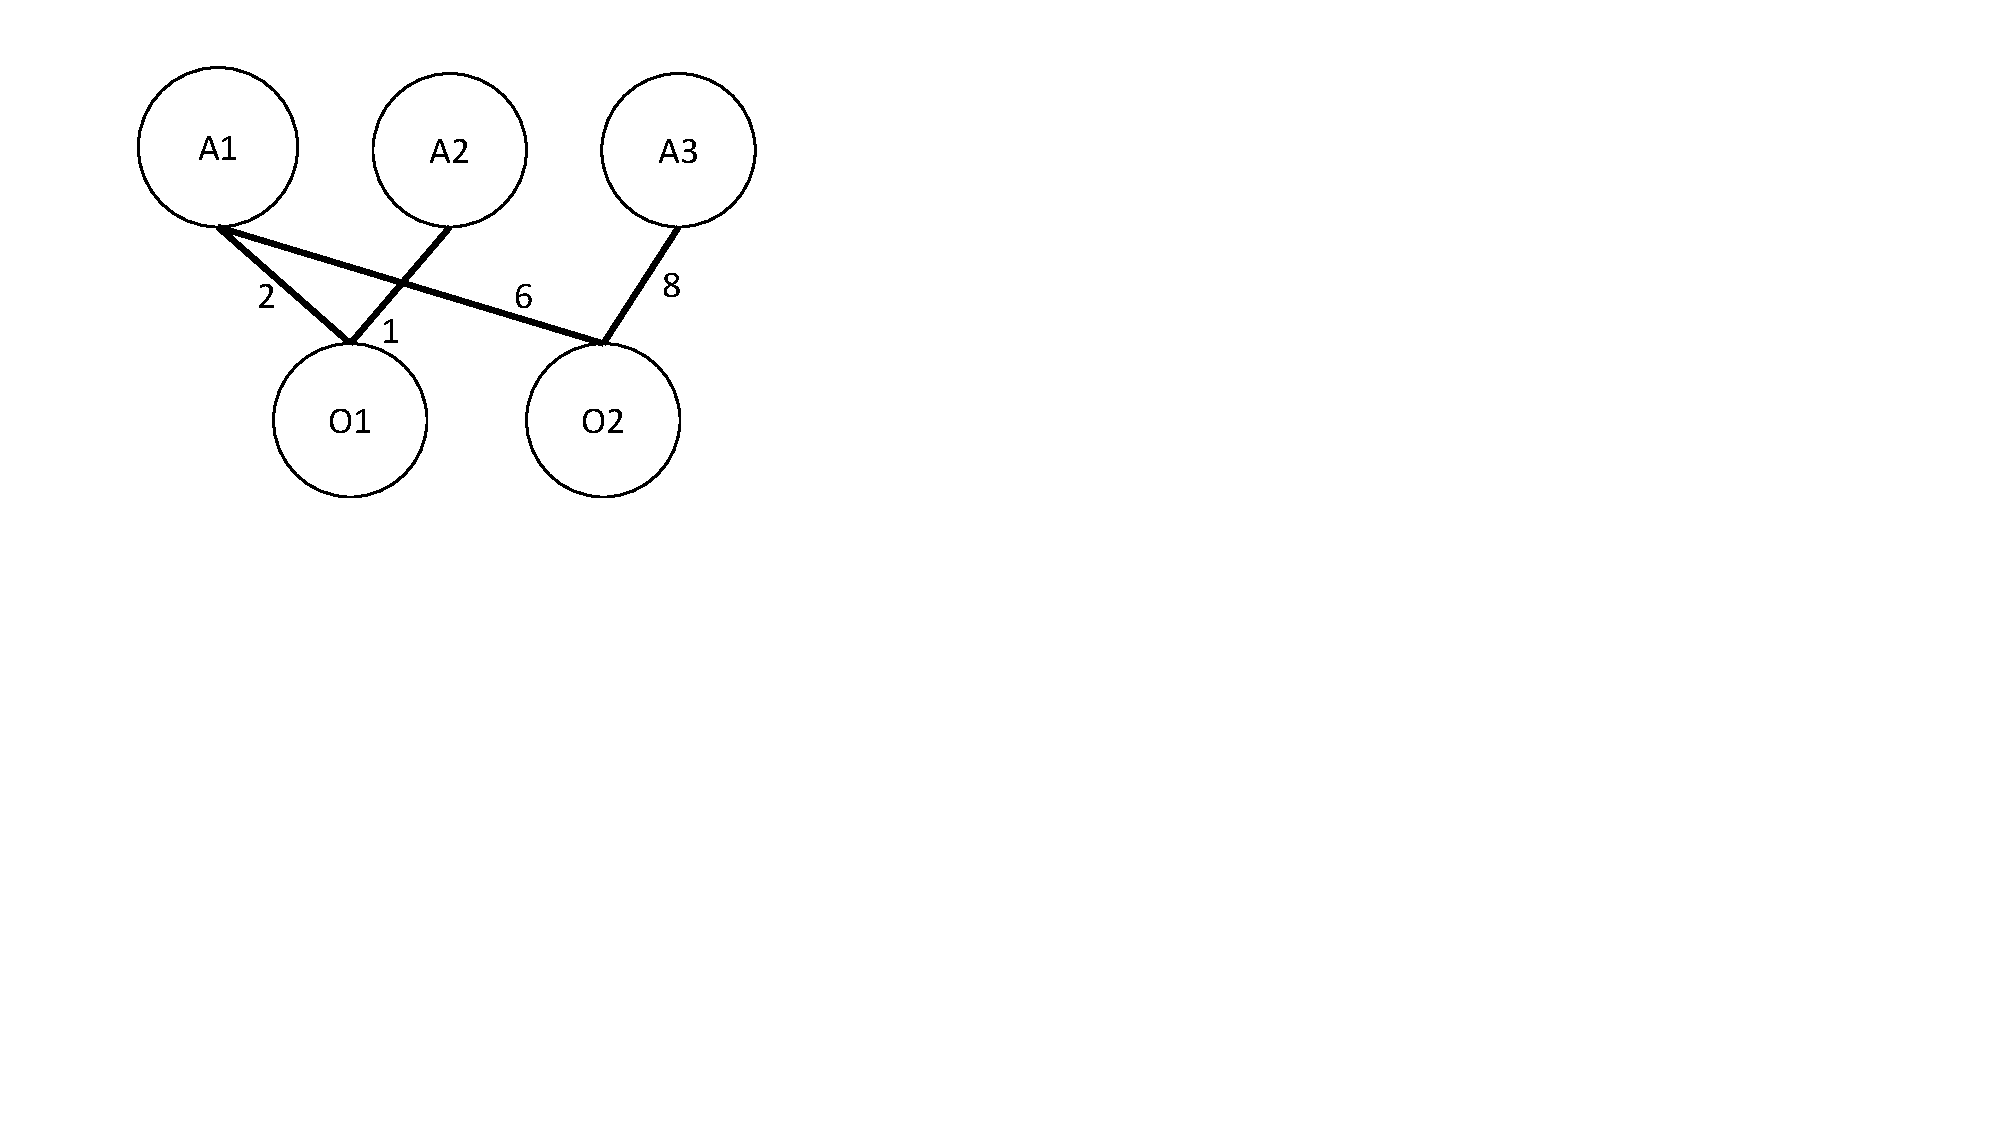
\includegraphics[width=10cm, trim={1.5cm 9.5cm 16.0cm 0cm}]{img/MatchCluster.pdf}
	\caption{Match Activity Cluster (A1-A3) and Object Cluster (O1-O2)}
	\label{fig:matchCluster}
\end{figure}

\noindent
Speaking the first approach, each data object cluster is simply matched to the activity cluster that is connected by the edge with the highest weight. Further, merge object clusters that match the same activity cluster. Activity clusters that have not been matched to a data object cluster remain without accompanying data objects, i.e. not merge with another activity cluster to avoid the combination of two different bounded contexts. Whereas this approach is straightforward and easy to apply, it has drawbacks: The cluster matching from data object point of view does not consider the overall dependencies. Regarding Fig.\ref{fig:matchCluster}, the result would be \textit{(O1,A1),(O2,A3),A2}. Despite the fact that \textit{A1} accesses \textit{O2} six times, it is outweighed by the combination (\textit{O2,A3}).  \\
The second approach is similar as each activity cluster is matched to the object cluster that is connected by the edge with the highest weight. Activity clusters that match the same object clusters are merged. Solely object clusters that remain unmatched in the end need to be matched with one of its connected activity clusters, as the data needs to be available somewhere. The best fit in regard to data accesses is the connected activity cluster node with the highest edge weight. In this case, the result obtained from Fig.\ref{fig:matchCluster} would be \textit{(A1,A3,O2),(A2,O1)}. Like the first approach, overall dependencies are not noticed. \\
In order to avoid this, i.e. to consider the dependencies holistically, the third approach uses the same clustering algorithm as proposed in Sec.\ref{sec:Solution:IdentifyCluster}. Thus, highly cohesive activity and data object clusters are combined. In regard to the running example \textit{CoCoME}, this approach provided satisfactory results. However, the clustering method usually merges activity clusters which can result in a too coarse-grained final microservice decomposition recommendation. So far, none of the approaches consider to split data object or activity clusters. For that, a closer look to the actual activity-data-relationships has to be taken. \\
In the following, we present a conceptual solution to match the two types of clusters according to their profound relationships. Hence, a white box approach is proposed: First, the clustering as presented previously is applied to achieve a first decomposition. As mentioned before, this step combines high cohesive data object clusters and activity clusters. In the next step, each combined cluster is scrutinized more precisely. In the situation that a combined cluster consists only of one activity and one data object cluster, there is nothing to do. If two (or more) activity clusters are merged and reference one data object cluster, it is necessary to take a closer look at the actual data objects they reference. In case both activity clusters reference mostly the same set of data objects in that cluster, merging is useful as distributing the activities in different services causes inevitable cross-service communication. Splitting object clusters is reasonable if it becomes apparent that one part of the data objects are referenced mostly by one activity cluster and the other part by the other activity clusters. Consequently, the previously identified set of activity clusters and the data cluster is divided into smaller parts while preserving the internal cohesion between data and activities and while keeping the combined cluster small. \\
This approach to match clusters is not yet mature and only presented conceptional. Neither a concise definition is provided nor has it been tested on several case studies. However, we believe in the potential of the cluster matching method and propose a more detailed case study in this area. Although we are aware that the third solution may produce too coarsely granular results, we chose this one, for now, to match the identified data object clusters and activity clusters. \\





\section{Extract Microservice Candidates}
\label{sec:Solution:ExtractMicroserviceCandidates}
So far, BPMN models are used to extract the control flow and the data flow from a system's business processes. Based on heuristics, we determine dependencies between the activities and between the data objects and visualize them as two graphs to identify clusters of dense relationships that are weakly connected to other clusters. In the previous section, we propose different approaches to match the activity clusters and the object clusters in order to obtain combined clusters. Those clusters correspond to the microservice candidates: The activities describe the functionality that the microservice provides. The data object clusters describe the data object which the microservice has to administer. The administration also includes the availability of interfaces to share data with other services if necessary.
Those combined clusters are good candidates to become a microservice, because:
\begin{itemize}
	\item Most of the data objects are accessed by activities within the service, which satisfies the low coupling criteria.
	\item Cohesive functionality is placed in the same service, which satisfies the high cohesion criteria.
	\item The approach reduces inter-service communication to a minimum, which enhances the performance.
\end{itemize}

This step finalizes the microservice identification approach. In the following, it is applied to CoCoME which is introduced in Chapter \ref{ch:CoCoME}. 










